\chapter{烃}
\section{有机物}
在日常生活和工农业生产里，人们从动物、植物等生物体中取得糖类、淀粉、蛋白质、油脂、纤维素和染料等等多种多样的化合物作为吃、穿、用等方面的必需品，已经有非常悠久的历史。
由于在那时这类化合物只能从动、植物等有机体中取得，因此人们就把这类化合物称为有机化合物。

从十九世纪二十年代开始，人们用非生物体内取得的物质先后合成了许多有机化合物，如尿素等。这样，就打破了只能从有机体取得有机化合物的限制。
现在，人们不但能够合成自然界里已有的许多种有机化合物，而且能够合成自然界里原来没有的多种多样性质良好的有机化合物，如合成树脂、合成橡胶、合成纤维和许多药物、染料等等。
因此“有机化合物”这个名称已失去了历史上原来的意义，只是因为大家习用这个名称，所以一直沿用着。

现在，我们所说的有机化合物，简称有机物，指的是含碳元素的化合物。
而把研究有机物的化学，叫做有机化学。
组成有机物的元素，除主要的碳外，通常还有氢、氧、氮、硫、卤素、磷等。
无机化合物，简称无机物\footnote{无机物里也包括单质。}，一般指的是组成里不含碳元素的物质。
我们过去已学过的很多化合物如水、食盐、氨、硫酸等等都是无机物。
而象一氧化碳、二氧化碳、碳酸盐等少数物质，虽然含有碳元素，但它们的组成和性质跟无机物很相近，一向把它们作为无机物。

有机物种类繁多，目前从自然界发现的和人工合成的有机物已达数百万种，而无机物却只有十来万种。
这是由于碳元素的原子的外层有四个价电子，可以跟其它原子形成四个共价键，而且更为突出的是碳原子跟碳原子之间能以比较稳定的共价键相结合，形成长的碳链。

一般说来，有机物具有以下主要特点。

大多数有机物难溶于水，易溶于汽油、酒精、苯等有机溶剂。
我们知道，许多无机物是易溶于水的。

绝大多数有机物受热容易分解，而且容易燃烧，而绝大多数无机物是不易燃烧的。

绝大多数有机物是非电解质，不易导电，熔点低。

有机物所起的化学反应比较复杂，一般比较慢，有的需要几小时甚至几天或更长时间才能完成，并且还常伴有副反应发生。
所以许多有机化学反应常常需要加热或应用催化剂以促进反应的进行。
这跟许多瞬时就可以完成的无机物的反应显然是不同的。

上面提到的有机化合物的许多物理性质和化学性质的特点，也是跟有机物的结构密切相关的。
大多数有机物分子里的碳原子跟其它原子经常是以共价键相结合，同时这些分子聚集时，又是分子晶体。
我们学习过的无机物许多是以离子键结合的，并形成离子晶体。
这些结构上的不同，就会在有机物的物理性质和化学性质方面表现出来。
当然严格来讲，有机物和无机物在性质上的区别也并不是绝对的。

由于有机物对发展国民经济和提高人民生活水平都具有重要意义，在近代，生产有机物的各种工业就越来越迅速地得到了发展。

有机化学早已从研究和利用天然有机物发展到大量用人工的方法制造（合成）新的有机物了。

有机化学在农业、能源、材料等科学技术研究领域里占有极为重要的地位。
有机化学也是研究跟生命有关的生物化学以及分子生物学的基础之一。

因此，学好有机化学，对于今后参加祖国的四个现代化建设是必要的。

\begin{Practice}[习题]
\begin{question}
  \item 什么叫有机物？组成有机物的元素主要的有哪几种？
  \item 简述有机物的特点。
\end{question}
\end{Practice}

\section{甲烷}
有机化合物里，有一大类物质是仅由碳和氢两种元素组成的,这类物质的总称叫烃\footnote{烃音\pinyin{ting1}。}，也叫碳氢化合物。
甲烷是烃类里分子组成最简单的物质。
\subsection{甲烷在自然界里的存在}
甲烷是没有颜色、没有气味的气体。
它的密度（在标准状况下）是 \qty{0.717}{g/L}，大约是空气密度的一半。
它极难溶解于水，很容易燃烧。

甲烷又叫沼气，也叫坑气。
这是因为池沼的底部和煤矿的坑道所产生的气体主要成分是甲烷的缘故。
这些甲烷都是在隔绝空气的情况下，由植物残体经过某些微生物发酵的作用而生成的。
此外，在有些地方的地下深处蕴藏着大量叫做天然气的可燃性气体，它的主要成分也是甲烷（按体积计，天然气里一般约含有甲烷  80\%～90\%，有的高达 98\%）。

沼气对于解决我国农村的能源问题，改善农村环境卫生，提高肥料质量等方面都有重要的意义。
近年来我国农村沼气的发展很快。

\subsection{甲烷分子的组成和结构}
甲烷由碳和氢两种元素组成。
根据标准状况下已测得甲烷气体的密度，我们可以计算出甲烷的摩尔质量约等于：
\[ \qty{0.717}{g/L} \times \qty{22.4}{L/mol} = \qty{16}{g/mol}\]

通过对甲烷气体进行的定量的测定，可以知道，甲烷里碳的百分含量是 75\%，氢的百分含量是 25\%。我们可以得出：

\qty{1}{mol} 甲烷分子里的含碳量约等于 $\qty{1}{mol} \times \qty{16}{g/mol}\times 75\%=\qty{12}{g}$。\qty{1}{mol} 碳原子的质量是 \qty{12}{g}，所以，\qty{1}{mol} 甲烷分子含 \qty{1}{mol} 碳原子。

\qty{1}{mol} 甲烷分子里的含氢量约等于 $\qty{1}{mol} \times \qty{16}{g/mol}\times 25\%=\qty{4}{g}$。\qty{1}{mol} 氢原子的质量是 \qty{1}{g}，所以，\qty{1}{mol} 甲烷分子含 \qty{4}{mol} 氢原子。

因此，甲烷的化学式是：\ce{CH4}。

那么，在甲烷分子里，1 个碳原子和 4 个氢原子是怎样结合的呢？要说明这个问题，让我们回忆碳原子核外电子排布的情况。碳原子的电子排布式是：$1s^22s^22p^2$，它的轨道表示式是：
\begin{figurehere}
  \includegraphics{2-a.pdf}
\end{figurehere}
它说明在碳原子的 4 个价电子里有两个 $2s$ 电子、两个 $2p$ 电子。
当碳原子参加化学反应时，1 个 $2s$ 电子在反应过程里吸收一定的能量，被激发到 $2p$ 轨道，这可表示如下：
\begin{figurehere}
  \includegraphics{2-b.pdf}
\end{figurehere}
这时,碳原子的未成对电子就是 1 个 $2s$ 电子和 3 个 $2p$ 电子。
因此，碳显示 4 价，它能跟 4 个氢原子形成 4 个共价键。
如果以 $\cdot$ 表示碳原子的价电子，以 $\scriptstyle\times$ 表示氢原子的价电子，甲烷的电子式可以写作：
\begin{figurehere}
  \includegraphics{2-c.pdf}
\end{figurehere}
在化学上常用一条短线来代表一对共用电子。
因此可以用下式来表示甲烷分子的结构：
\[ \chemfig{H-C(-[:90]H)(-[:-90]H)-H}\]

这种用短线来代表一对共用电子的图式叫做\Concept{结构式}。

甲烷的结构式虽然可以初步说明碳原子跟氢原子间的结合情况，但是并不能够说明分子里各原子在空间分布的实际情况。
经过大量的科学实验证明，甲烷分子里的一个碳原子和四个氢原子不在同一个平面上，而是形成了一个正四面体的立体结构。
碳原子位于正四面体的中心，而四个氢原子分别位于正四面体的四个顶点上。
碳原子的四个价键之间的夹角（键角）彼此相等，都是 \ang{109;28;}。
四个碳氢键的键长都是 \qty{1.09e-10}{m}。
经测定，\ce{C-H} 键的键能是 \qty{98.8}{kCal/mol}。
\cref{fig:2-1} 是甲烷分子结构的示意图，它可以表示分子里各原子的相对位置。
\cref{fig:2-2a} 是甲烷分子的一种模型，黑球代表碳原子，白球代表氢原子，短棍代表价键。这种模型叫做球棍模型。
\cref{fig:2-2b} 是甲烷分子的另一种模型，叫做比例模型。它用黑球和白球的体积比，来大体上表示碳氢两种原子的体积比。
\begin{figure}
  \begin{minipage}[b]{0.4\linewidth}\centering
    \includegraphics{2-1.pdf}
    \caption{甲烷分子结构的示意图}\label{fig:2-1}
  \end{minipage}%
  \begin{minipage}[b]{0.6\linewidth}
    \nextfloat
    \begin{subfigure}{0.48\linewidth}\centering
      \includegraphics{2-2a.pdf}
      \caption{球棍模型}\label{fig:2-2a}
    \end{subfigure}%
    \begin{subfigure}{0.48\linewidth}\centering
      \includegraphics{2-2b.pdf}
      \caption{比例模型}\label{fig:2-2b}
    \end{subfigure}
    \caption{甲烷分子的模型}\label{fig:2-2}
  \end{minipage}
\end{figure}

化合物的结构式对于我们认识它们的结构、制法、性质等都是很重要的，对于有机化合物更是这样。
表示分子结构的模型可以帮助我们进一步了解分子的立体形状和分子内各原子的相对位置。
对此我们将在以后作进一步的介绍。

有机物的立体结构书写起来比较费事，为方便起见，一般仍采用平面的结构式。

\begin{Reading}[补充阅读]{}
甲烷分子为什么有这样的结构呢？

我们知道，在甲烷分子里碳原子参加化学反应时，由于一个 $2s$ 电子被激发到 $2p$ 轨道，这样就有了 4 个不成对的最外层电子，因此碳原子显示 4 价。

但是，我们知道，$2s$ 电子和 $2p$ 电子是有区别的，由此推测在甲烷分子里的四个价键不可能完全相同，其中一个键应当不同于另外的三个键。
但是实验事实证明，所有这四个键是等同的。
这是什么道理呢？为了解释这个矛盾，人们提出了杂化轨道的理论。

这个理论认为，在甲烷分子里，碳原子的四个能成锭的电子，并不是分别占有 $2s$、$2p_x$、$2p_y$、$2p_z$ 轨道，而是由这四个轨道“混和”起来，重新组合成四个能量等同的新轨道。
这种组合成新轨道的过程就叫做\Concept{杂化}。
由一个 $s$ 轨道和三个 $p$ 轨道杂化形成的四个新轨道叫做 $sp^3$ 杂化轨道。
对于碳原子来说，这种杂化轨道（如果同时考虑轨道的能量差别）可以表示为：
\begin{figurehere}
  \includegraphics{2-d.pdf}
\end{figurehere}

碳原子的一个 $sp^3$ 杂化轨道表示如\cref{fig:2-3a}。
它的四个 $sp^3$ 杂化轨道指向正四面体的四个顶点。 $sp^3$ 杂化轨道对称轴间的夹角是 \ang{109;28;}。碳原子位于正四面体的中心（\cref{fig:2-3b}）。
\begin{figurehere}
  \begin{minipage}[b]{0.56\linewidth}
    \nextfloat
    \begin{subfigure}{0.48\linewidth}\centering
      \includegraphics{2-3a.pdf}
      \caption{一个 $sp^3$ 杂化轨道}\label{fig:2-3a}
    \end{subfigure}%
    \begin{subfigure}{0.48\linewidth}\centering
      \includegraphics{2-3b.pdf}
      \caption{四个 $sp^3$ 杂化轨道}\label{fig:2-3b}
    \end{subfigure}
    \caption{碳原子的 $sp^3$ 杂化}\label{fig:2-3}
  \end{minipage}%
  \begin{minipage}[b]{0.44\linewidth}\centering
    \includegraphics{2-4.pdf}
    \caption{碳原子跟氢原子的轨道重叠}\label{fig:2-4}
  \end{minipage}
\end{figurehere}

根据杂化轨道理论，我们可以认为: 甲烷分子里四个 $sp^3$ 杂化轨道分别跟四个氢原子的 $1s$ 轨道重叠形成四个 \ce{C-H} 共价键。
由于 $sp^3$ 杂化轨道的形状是一头大一头小的，大的一头可以跟另一原子的轨道重叠，这样重叠的效果较好，成键能力也较大（\cref{fig:2-4}）。

这种由两个相同或不相同的原子的价电子沿着轨道对称轴（这里就是连接两原子核的直线）方向相互重叠所形成的键，叫做 $\sigma$ 键 \footnote{$\sigma$ 音 /sigma/。}。$\sigma$ 键的特点是能够围绕对称轴旋转，而不影响键的强度和键跟键之间的角度，如氢分子中的 \ce{H-H} 键，氯化氢分子中的 \ce{H-Cl} 键和甲烷分子中的 \ce{C-H} 键，都是 $\sigma$ 键。
\end{Reading}

\subsection{甲烷的制法和性质}
\subsubsection{甲烷的制法}
在实验室里，甲烷是用无水醋酸钠（\ce{CH3COONa}）和碱石灰混和加热制得的（见\cref{fig:2-5},\MyRoman{1}）。
碱石灰是氢氧化钠和石灰的混和物，氢氧化钠跟醋酸钠起反应的化学方程式\footnote{有机物参加的化学反应往往比较复杂，常有副反应发生等。因此，有关有机物反应的化学方程式通常不用等号而用箭号 \ce{->} 表示。} 如下：
\[
\schemestart
\chemname{\chemfig{CH_3COONa}}{\footnotesize 醋酸钠}
\+
\chemfig{NaOH}
\arrow(.mid east--.mid west){->[$\triangle$]}
\chemfig{Na_2CO_3}
\+
\chemname{\chemfig{CH_4}}{\footnotesize 甲烷} \ce{ ^ }
\schemestop\chemnameinit{}
\]

\begin{Experiment}
取一药匙研细的无水醋酸钠和三药匙研细的碱石灰 \footnote{碱石灰可以用适量的氢氧化钙和氧化钙的混合物代替。}，在纸上充分混和，迅速装进试管，装置如\cref{fig:2-5},\MyRoman{1} 所示。加热。用排水集气法把甲烷收集在试管里。观察它的颜色和闻它的气味。
\tcblower
\begin{figurehere}
  \includegraphics{2-5.pdf}\par
  {\footnotesize \begin{enumerate*}[I] \item 制取甲烷\quad\mbox{} \item 甲烷的燃烧\quad\mbox{} \item 甲烷通入高锰酸钾溶液 \end{enumerate*}}
  \caption{甲烷的制取和性质}\label{fig:2-5}
\end{figurehere}
\end{Experiment}

\subsubsection{甲烷的化学性质和用途}
在通常情况下，甲烷是比较稳定的，跟强酸、强碱或强氧化剂等一般不起反应。
\begin{Experiment}
  把甲烷经导管通入盛有高锰酸钾酸性溶液的试管里（\cref{fig:2-5},\MyRoman{3}），观察紫色溶液是否有变化。
\end{Experiment}
我们从实验看到，溶液颜色没有变化，说明甲烷跟强氧化剂高锰酸钾不起反应。
但是甲烷的稳定性是相对的，在特定的条件下，也会发生某些反应。

\paragraph{取代反应}\mbox{}\par
\begin{Experiment}
制备好一集气瓶的纯净的甲烷和氯气的混和气体，用玻璃片把瓶口盖好，放在光亮的地方（注意: 不要放在日光直射的地方，否则会引起爆炸）。等待片刻，观察瓶内气体颜色的变化。
\end{Experiment}
在室温下，甲烷和氯气的混和物可以在黑暗中长期保存而不起任何反应。
但把混和气体放在光亮的地方就会发生反应，黄绿色的氯气就会逐渐变淡。
这个反应的化学方程式可以表示如下（为明显起见，用结构式代替化学式）：
\[ 
\schemestart
\chemfig{H-C(-[:90]H)(-[:-90]H)-H}\tikz[remember picture,overlay] \coordinate (a); 
\+
\tikz[remember picture,overlay] \coordinate (b); 
\chemfig{Cl-Cl}
\arrow(.mid east--.mid west){->[{\scriptsize 光}]}
\chemname{\chemfig{H-C(-[:90]H)(-[:-90]H)-Cl}}{\footnotesize 一氯甲烷}
\+ 
\chemfig{H-Cl}
\schemestop\chemnameinit{}
\tikz[remember picture,overlay] \draw[densely dashed] ([xshift=-1.3em,yshift=-1ex]a)rectangle([xshift=1.8em,yshift=1em]b); 
\]

但是反应并没有停止，生成的一氯甲烷仍继续跟氯气作用，依次生成二氯甲烷、三氯甲烷（又叫氯仿）和四氯甲烷（又叫四氯化碳）。
反应分别表示如下：
\[ 
\schemestart
\chemfig{H-C(-[:90]H)(-[:-90]Cl)-H}\tikz[remember picture,overlay] \coordinate (a); 
\+
\tikz[remember picture,overlay] \coordinate (b);
\chemfig{Cl-Cl}
\arrow(.mid east--.mid west){->[{\scriptsize 光}]}
\chemname{\chemfig{H-C(-[:90]H)(-[:-90]Cl)-Cl}}{\footnotesize 二氯甲烷}
\+ 
\chemfig{H-Cl}
\schemestop\chemnameinit{}
\tikz[remember picture,overlay] \draw[densely dashed] ([xshift=-1.3em,yshift=-1ex]a)rectangle([xshift=1.8em,yshift=1em]b); 
\]
\[ 
\schemestart
\chemfig{Cl-C(-[:90]H)(-[:-90]Cl)-H}\tikz[remember picture,overlay] \coordinate (a);  
\+
\tikz[remember picture,overlay] \coordinate (b);
\chemfig{Cl-Cl}
\arrow(.mid east--.mid west){->[{\scriptsize 光}]}
\chemname{\chemfig{Cl-C(-[:90]H)(-[:-90]Cl)-Cl}}{\footnotesize 三氯甲烷}
\+ 
\chemfig{H-Cl}
\schemestop\chemnameinit{}
\tikz[remember picture,overlay] \draw[densely dashed] ([xshift=-1.3em,yshift=-1ex]a)rectangle([xshift=1.8em,yshift=1em]b); 
\]
\[ 
\schemestart
\chemfig{Cl-C(-[:90]Cl)(-[:-90]Cl)-H}\tikz[remember picture,overlay] \coordinate (a);  
\+
\tikz[remember picture,overlay] \coordinate (b);
\chemfig{Cl-Cl}
\arrow(.mid east--.mid west){->[{\scriptsize 光}]}
\chemname{\chemfig{Cl-C(-[:90]Cl)(-[:-90]Cl)-Cl}}{\footnotesize 四氯甲烷}
\+ 
\chemfig{H-Cl}
\schemestop\chemnameinit{}
\tikz[remember picture,overlay] \draw[densely dashed] ([xshift=-1.3em,yshift=-1ex]a)rectangle([xshift=1.8em,yshift=1em]b); 
\]

在这些反应里，甲烷分子里的氢原子逐步被氯原子所代替而生成了四种取代产物。
\emph{有机物分子里的某些原子或原子团被其它原子或原子团所代替的反应叫做}\Concept{取代反应}。

一氯甲烷等四种取代产物都是甲烷的氯代物。
它们都不溶于水。
在常温一氯甲烷是气体，其它三种都是液体。
三氯甲烷和四氯甲烷都是工业上重要的溶剂。
四氯甲烷还是一种效率较高的灭火剂。

\paragraph{氧化反应}\mbox{}\par
\begin{Experiment}
点燃纯净的甲烷（注意：点燃前必须象检验氢气纯度那样先检验甲烷的纯度），注意观察火焰。然后在火焰上方罩一个干燥的烧杯（\cref{fig:2-5}，\MyRoman{2}），很快就可以看见烧杯内壁变得摸糊，并有水蒸气凝结。
把烧杯倒转过来，向杯内注入少量澄清石灰水，振荡，观察石灰水变浑浊。
\end{Experiment}
纯净的甲烷在空气里安静地燃烧，生成二氧化碳和水，同时放出大量的热。
\[ \ce{ CH4 +2O2 ->[\text{点燃}] CO2 + 2H2O \text{（液）} + \qty{212.8}{kCal} }\]

甲烷是一种很好的气体燃料。
但是必须注意，如果点燃甲烷跟氧气或空气的混和物\footnote{甲烷在空气里的爆炸极限是含甲烷 5\%～15\%，在氧气里的爆炸极限是 5.4\%～59.2\%。}，它就立即发生爆炸。
因此，在煤矿的矿井里，必须采取安全措施，如通风、严禁烟火等，以防止甲烷跟空气混和物的爆炸事故发生。

\paragraph{加热分解}\mbox{}\par
在隔绝空气的条件下加热到将近 \qty{1000}{\celsius}，甲烷就开始分解；加热时间较长，到 \qty{1500}{\celsius} 左右，分解比较完全，生成炭黑和氢气。
\[ \ce{ CH4 ->[\text{高温}] C + 2H2 ^}\]

甲烷分解生成的炭黑是橡胶工业的重要原料，也可以用于制造颜料、油墨、油漆等，生成的氢气可作合成氨的原料。

\begin{Practice}[习题]
\begin{question}
  \item 某气体含碳 82.7\%，含氢 17.3\%，在标准状况下，它的密度是 \qty{2.59}{g/L}。求这种气体的化学式。
  \item 已知一种烃含碳 92.3\%，含氢 7.7\%，在 \qty{1}{atm} 和 \qty{117}{\celsius} 温度时，该化合物（蒸气）\qty{0.5}{g} 占体积 \qty{205}{ml}。求这种烃的式量和化学式。
  \item 怎样用实验来鉴别甲烷、氢气和一氧化碳？
  \item 溴跟甲烷的取代反应和产物同氯气跟甲烷的取代反应和产物相类似。写出溴跟甲烷起反应的各步化学方程式。
  \item 当温度是 \qty{27}{\celsius}，压强是 \qty{750}{mmHg} 时，\qty{5}{mol} 甲烷发生燃烧，能生成多少升的二氧化碳？
\end{question}
\end{Practice}

\section{烷烃\texorpdfstring{\quad}{ }同系物}
\subsection{烷烃}
除甲烷外，还有一系列性质跟它很相似的烃，像乙烷（\ce{C2H5}）、丙烷（\ce{C3H8}）、丁烷（\ce{C4H10}）等等。它们的结构式可以分别表示如下：
\[
\schemestart
\chemname{\chemfig{H-C(-[:90]H)(-[:-90]H)-C(-[:90]H)(-[:-90]H)-H}}{\footnotesize 乙烷}\qquad
\chemname{\chemfig{H-C(-[:90]H)(-[:-90]H)-C(-[:90]H)(-[:-90]H)-C(-[:90]H)(-[:-90]H)-H}}{\footnotesize 丙烷}\qquad
\chemname{\chemfig{H-C(-[:90]H)(-[:-90]H)-C(-[:90]H)(-[:-90]H)-C(-[:90]H)(-[:-90]H)-C(-[:90]H)(-[:-90]H)-H}}{\footnotesize 丁烷}
\schemestop\chemnameinit{}
\]

在这些烃的分子里，碳原子跟碳原子都以单键结合成链状，跟甲烷一样，碳原子剩余的价键全部跟氢原子相结合。
这样的结合使得每个碳原子的化合价都已充分利用，都达到“饱和”。
具有这种结合的链烃叫做\Concept{饱和链烃}，或称\Concept{烷烃}。

这些烷烃是根据分子里所含的碳原子的数目来命名的。
碳原子数在十以下的，从一到十依次用甲、乙、丙、丁、戊、己、庚、辛、壬、癸来表示，碳原子数在十一以上的，就用数字来表示。
例如，\ce{C7H16} 叫庚烷，\ce{C17H36} 叫十七烷。

为了书写方便，有机物除用结构式表示外，也可以用结构简式表示。
如乙烷的结构简式是 \ce{CH3CH3}，丙烷的结构简式是 \ce{CH3CH2CH3}，戊烷的结构简式是 \ce{CH3(CH2)3CH3}，等等。

烷烃的种类很多，\cref{tab:2-1} 里只列出其中的一部分。
\begin{table}
  \caption{几种烷烃的物理性质}\label{tab:2-1}
  \begin{tblr}{colspec={cX[l]cS[table-format=5.2]S[table-format=5.2]l},hline{2}=0.8pt,row{1}={m,c,guard}}
    名称 & 结构简式 & {常温时\\状态} & 熔点 \unit{\celsius} & 沸点 \unit{\celsius} & {液态时的密度\\（\unit{g/cm^3}）}\\
    甲烷 & \ce{CH4}               & 气 & -182.5 & -164   & $0.466^*$ \\
    乙烷 & \ce{CH3CH3}            & 气 & -183.3 & -88.63 & $0.572^{**}$ \\
    丙烷 & \ce{CH3CH2CH3}         & 气 & -189.7 & -42.07 & $0.5005$ \\
    丁烷 & \ce{CH3(CH2)2CH3}      & 气 & -138.4 & -0.5   & $0.5788$ \\
    戊烷 & \ce{CH3(CH2)3CH3}      & 液 & -129.7 & 36.07  & $0.6262$ \\
    庚烷 & \ce{CH3(CH2)5CH3}      & 液 & -90.61 & 98.42  & $0.6838$ \\
    辛烷 & \ce{CH3(CH2)6CH3}      & 液 & -56.79 & 125.7  & $0.7025$ \\
    癸烷 & \ce{CH3(CH2)8CH3}      & 液 &  -29.7 & 174.1  & $0.7300$ \\
    十七烷 & \ce{CH3(CH2)15CH3}   & 固 & 22     & 301.8  & $0.7780$（固态）\\
    二十四烷 & \ce{CH3(CH2)22CH3} & 固 & 54     & 391.3  & $0.7991$（固态）\\
  \end{tblr}\par
  \begin{minipage}{\linewidth}
    \footnotesize * 是 \qty{-64}{\celsius} 时的值，** 是 \qty{-108}{\celsius} 时的值，其余是 \qty{20}{\celsius} 时的值。
  \end{minipage}
\end{table}

\subsection{同系物}
从\cref{tab:2-1} 还可以看出，各种烷烃的物理性质一般随着分子里碳原子数的递增（同时式量也在递增），发生规律性的变化。
例如，在常温下，它们的状态是由气态、液态到固态；它们的沸点逐渐增加。

这些烃在化学性质上跟甲烷相似。
在通常状况下，它们很稳定，跟酸、碱和氧化剂都不起反应，也难于跟其它物质化合。
这些烃在空气里都可以点燃。
在光照条件下，这些烃都能跟氯气起取代反应等。

从\cref{tab:2-1} 里的烷烃化学式可以看出，相邻两个烷烃在组成上都相差一个“\ce{CH2}”原子团。
如果把碳原子数定为 $n$，氢原子数就是 $2n+2$。
所以烷烃的化学式可用通式 \ce{C_$n$H_$2n+2$} 来表示。

我们把\emph{结构相似，在分子组成上相差一个或若干个 \ce{CH2} 原子团的物质互相称为}\Concept{同系物}。

甲烷、乙烷、丙烷等都是烷烃的同系物。

\subsection{烃基}
烃分子失去一个或几个氢原子后所剩余的部分叫做\Concept{烃基}。
烃基一般用“\ce{R-{}}”表示。
如果这种烃是烷烃，那么烷烃失去氢原子后所剩余的原子团叫做烷基。
\ce{-CH3} 叫甲基，\ce{-CH2CH3} 叫乙基等。

\subsection{同分异构体\texorpdfstring{\quad}{ }烷烃的命名}
\subsubsection{同分异构现象}
在研究物质的分子组成和性质时，发现有很多物质的分子组成相同，但性质却有差异。
例如，在研究丁烷（\ce{C4H10}）的组成和性质的过程里，发现有另一种组成和式量跟丁烷完全相同，但性质却有差异的物质。
为了区别起见，人们把一种叫做正丁烷，另一种叫做异丁烷。
现在把它们在性质上的差异略举几例如下：

\begin{tblr}{colspec={rS[table-format=9.4]S[table-format=9.4]},hlines=0pt,vlines=0pt,row{1}={m,c,guard}}
  & 正丁烷 & 异丁烷 \\
  熔点（\unit{\celsius}）& -138.4 & -159.6 \\
  沸点（\unit{\celsius}）& -0.5 & -11.7 \\
  液态时的密度（\unit{g/cm^3}）& 0.5788 & 0.557 \\
\end{tblr}

为什么这两种丁烷具有相同的组成和相同的式量但却有不同的性质呢？经过科学实验证明，原来它们的结构是不同的。
正丁烷分子里的碳原子形成直链，而异丁烷分子里的碳原子却带有支链：
\[
\schemestart
\chemname{\chemfig{H-C(-[:90]H)(-[:-90]H)-C(-[:90]H)(-[:-90]H)-C(-[:90]H)(-[:-90]H)-C(-[:90]H)(-[:-90]H)-H}}{\footnotesize 正丁烷}\qquad
\chemname{\chemfig{H-C(-[:90]H)(-[:-90]H)-[::0,1.5]C(-[:90]H)(-[::-90,1.5]C(-[:180]H)(-[:-90]H)-H)-[::0,1.5]C(-[:90]H)(-[:-90]H)-H}}{\footnotesize 异丁烷}
\schemestop\chemnameinit{}
\]

由此可见，烃分子里的碳原子既能形成直链的碳链（如正丁烷），又能形成带有支链的碳链。
因此虽然两种丁烷的组成相同，即化学式相同，但分子里原子结合的顺序不同，也就是说分子的结构不同，因此它们的性质就有差异。

\emph{化合物具有相同的化学式，但具有不同结构的现象，叫做}\Concept{同分异构现象}。
具有同分异构现象的化合物互称为同分异构体。
例如正丁烷和异丁烷就是丁烷的两种同分异构体。
戊烷有三种同分异构体。
戊烷的三种同分异构体的结构式如下：
\[
\schemestart
\chemname{\chemfig{H-C(-[:90]H)(-[:-90]H)-C(-[:90]H)(-[:-90]H)-C(-[:90]H)(-[:-90]H)-C(-[:90]H)(-[:-90]H)-C(-[:90]H)(-[:-90]H)-H}}{\footnotesize 正戊烷（沸点 \qty{36.07}{\celsius}）}
\qquad 
\chemname{\chemfig{H-C(-[:90]H)(-[:-90]H)-C(-[:90]H)(-[:-90]H)-[::0,1.5]C(-[:90]H)(-[::-90,1.5]C(-[:180]H)(-[:-90]H)-H)-[::0,1.5]C(-[:90]H)(-[:-90]H)-H}}{\footnotesize 异戊烷（沸点 \qty{27.9}{\celsius}）}
\schemestop\chemnameinit{}
\]
\[
\schemestart
\chemname{\chemfig{H-C(-[:90]H)(-[:-90]H)-[::0,1.5]C(-[::90,1.5]C(-[:180]H)(-[:90]H)-H)(-[::-90,1.5]C(-[:180]H)(-[:-90]H)-H)-[::0,1.5]C(-[:90]H)(-[:-90]H)-H}}{\footnotesize 新戊烷（沸点 \qty{9.5}{\celsius}）}
\schemestop\chemnameinit{}
\]

\cref{fig:2-6} 是戊烷的三种同分异构体的球棍模型。
\begin{figure}
  \begin{minipage}[b]{0.32\linewidth}\centering
    \includegraphics{2-6a.pdf}
    \subcaption{正戊烷}\label{fig:2-6a}
  \end{minipage}
  \begin{minipage}[b]{0.32\linewidth}\centering
    \includegraphics{2-6b.pdf}
    \subcaption{异戊烷}\label{fig:2-6b}
  \end{minipage}
  \begin{minipage}[b]{0.32\linewidth}\centering
    \includegraphics{2-6c.pdf}
    \subcaption{新戊烷}\label{fig:2-6c}
  \end{minipage}
  \caption{戊烷同分异构体分子的球棍模型}\label{fig:2-6}
\end{figure}

从\cref{fig:2-6} 可以看出，就是不带支链的链烃，它的碳链也不是直线形的，而是锯齿形的。
同样，异戊烷的分子里的碳链也是锯齿形的。

在烷烃同系物的分子里，随着碳原子数目的增多，碳原子间的结合方式就越趋复杂，同分异构体的数目也就越多。
例如己烷（\ce{C6H14}）有五种同分异构体，庚烷（\ce{C7H16}）有九种，而癸烷 （\ce{C10H22}）有 75 种之多。

\subsubsection{烷烃的命名法}
有机物种类繁多，分子的组成和结构又比较复杂，所以有机物的命名就显得十分重要。
前面提到的戊烷的三种同分异构体就只能用正、异、新来区别。
如果碳原子数目再多一些，这样简单的命名方法显然就不能满足需要。
现在我们以一个带有支链的烷烃为例，来介绍一种通用的系统命名法，这种命名法的步骤如下：
\begin{enumerate}
  \item 选定分子里最长的碳链做主链，并按主链上碳原子的数目称为“某烷”。
  \item 把主链里离支链较近的一端作为起点，用 $1,2,3,\dots\dots$ 等数字给主链的各个碳原子依次编号定位以确定支链的位置。
  \[ 
  \chemfig{\charge{90[anchor=-90]={\tiny 1}}{C}H_3-\charge{90[anchor=-90]={\tiny 2}}{C}H(-[:-90]CH_3)-\charge{90[anchor=-90]={\tiny 3}}{C}H_2-\charge{90[anchor=-90]={\tiny 4}}{C}H_3} \qquad\qquad
  \chemfig{\charge{90[anchor=-90]={\tiny 1}}{C}H_3-\charge{45[anchor=-135]={\tiny 2}}{C}(-[:90]CH_3)(-[:-90]CH_3)-\charge{90[anchor=-90]={\tiny 3}}{C}H_3}
  \]
  \item 把支链作为取代基。把取代烃基的名称写在烷烃名称的前面，在取代烃基的前面用阿拉伯数字注明它在烷烃直链上的所在位置，并在号数后面连一短线，中间用“-”隔开。 例如：
  \[ 
  \chemfig{\charge{90[anchor=-90]={\tiny 1}}{C}H_3-\charge{90[anchor=-90]={\tiny 2}}{C}H(-[:-90]CH_3)-\charge{90[anchor=-90]={\tiny 3}}{C}H_2-\charge{90[anchor=-90]={\tiny 4}}{C}H_3} \qquad\text{\footnotesize 2-甲基丁烷（即异戊烷）}
  \]
  \item 如果有相同的取代烃基，可以合并起来用二、三等数字表示，但表示相同取代烃基位置的阿拉伯数字要用“，”号隔开；如果几个取代烃基不同，就把简单的写在前面，复杂的写在后面。例如：
  \[
  \schemestart
  \chemname{\chemfig{\charge{90[anchor=-90]={\tiny 1}}{C}H_3-\charge{90[anchor=-90]={\tiny 2}}{C}H(-[:-90]CH_3)-\charge{90[anchor=-90]={\tiny 3}}{C}H(-[:-90]CH_3)-\charge{90[anchor=-90]={\tiny 4}}{C}H_2-\charge{90[anchor=-90]={\tiny 5}}{C}H_3}}{\footnotesize 2,3-二甲基戊烷}\qquad
  \chemname{\chemfig{\charge{90[anchor=-90]={\tiny 7}}{C}H_3-\charge{90[anchor=-90]={\tiny 6}}{C}H_2-\charge{90[anchor=-90]={\tiny 5}}{C}H_2-\charge{90[anchor=-90]={\tiny 4}}{C}H_2-\charge{90[anchor=-90]={\tiny 3}}{C}H(-[:-90]CH_3-[:-90]CH_3)-\charge{60[anchor=-120]={\tiny 2}}{C}H(-[:90]CH_3)-\charge{90[anchor=-90]={\tiny 1}}{C}H_3}}{\footnotesize 2-甲基-3-乙基庚烷}
  \schemestop\chemnameinit{}
  \]
\end{enumerate}

\subsection{环烷烃}
\emph{烃分子里碳原子间相互联接成环状的，叫做}\Concept{环烃}。

在环烃分子里，碳原子之间以单键相互结合的叫做环烷烃。环烷烃的性质跟饱和链烃相似。以下是四种环烷烃的结构简式。
\[
\schemestart
\chemname{\chemfig{H_2C*3(-CH_2-C(-[:180,0.5,,,draw=none]H_2)-)}}{\footnotesize 环丙烷}\qquad
\chemname{\chemfig{C*4(-CH_2-CH_2-C(-[:180,0.5,,,draw=none]H_2)-)(-[:180,0.5,,,draw=none]H_2)}}{\footnotesize 环丁烷}\qquad
\chemname{\chemfig{H_2C*5(-C(-[:-90,0.5,,,draw=none]H_2)-CH_2-C(-[:90,0.5,,,draw=none]H_2)-H_2C-[,,2])}}{\footnotesize 环戊烷}\qquad
\chemname{\chemfig{H_2C*6(-C(-[:-90,0.5,,,draw=none]H_2)-CH_2-[,,1,1]CH_2-C(-[:90,0.5,,,draw=none]H_2)-H_2C-[,,2])}}{\footnotesize 环己烷}
\schemestop\chemnameinit{}
\]

可以看出，环烷烃在分子的组成上比相应的烷烃少两个氢原子，所以环烷烃的通式是 \ce{C_$n$H_$2n$}。

在环烷烃里，工业上用途较广的有环己烷。环己烷是无色液体，易挥发，易燃烧，是生产合成纤维——锦纶的一种重要原料，也是一种有机溶剂。

\begin{Practice}[习题]
\begin{question}
  \item 什么叫同系物？写出下列各种直链烷烃的化学式和结构简式：
  \begin{tasks}(4)
    \task 辛烷，
    \task 十八烷，
    \task 二十三烷，
    \task 三十九烷，
    \task! 含有 30 个氢原子的烷。
  \end{tasks}
  \item 哪一种烷烃的密度跟空气的密度大体相近？
  \item 写出下面这种烃的名称。
  \[\chemfig{CH_3-CH(-[:90]CH_3)-CH_2-CH(-[:-90]CH_3)-CH_2-CH(-[:-90]CH_2-[:-90]CH_3)-CH_2-CH(-[:90]CH_2-[:90]CH_3)-CH_3}\]
  \item 写出戊烷的电子式。
  \item 写出已烷的各种同分异构体的结构简式，并用系统命名法命名。
  \item 燃烧 \qty{8.8}{g} 某气态烃，得到 \qty{26.4}{g} 二氧化碳。已知该烃的密度在标准状况下是 \qty{1.96}{g/L}，求该烃的化学式。
  \item 在标准状况下使 \qty{2}{mol} 甲烷跟 \qty{10}{L} 乙烷的混和气体完全燃烧，需要多少升空气？
  \item 写出辛烷完全燃烧的化学方程式。
  \item 同系物、同分异构体、同素异形体、同位素这四个名词的含义有什么不同？举例说明。
  \item 在下列的几种烷烃分子里，\CJKunderline*[hidden]{\hspace{1em}A、B、C\hspace{1em}}互为同分异构体。
  \begin{tasks}[label=\Alph*.](2)
    \task \ce{CH3CH2CH2CH2CH3}
    \task \ce{CH3CH(CH3)CH2CH3}
    \task \ce{(CH3)2CHCH2CH3}
    \task \ce{(CH3)2CHCH3}
    \task \ce{CH3CH2CH2CH2CH(CH3)2}
  \end{tasks}
  \item 写出下列各化合物的结构式：
  \begin{tasks}
    \task 2,5-二甲基庚烷，
    \task 2,3-二甲基-5-乙基辛烷。
  \end{tasks}
  \item 已知某种烃含碳 85.7\%，含氢 14.3\%，在标准状况下它的密度是 \qty{1.25}{g/L}。试求这种烃的式量和化学式。
\end{question}
\end{Practice}


\section[乙烯]{乙烯\texorpdfstring{\protect\footnote{烯音\pinyin{xi1}。}}{}}
在具有链状分子结构的烃里，除了饱和链烃外，还有许多烃，它们分子里的碳原子所结合的氢原子数少于饱和链烃里的氢原子数。
如果这些化合物跟某些物质起反应，它们分子里的这种碳原子还可以结合其它的原子或原子团。
通常把这类烃叫做不饱和烃。

乙烯就是一种不饱和烃。乙烯的化学式是 \ce{C2H4}，电子式和结构式是：
\[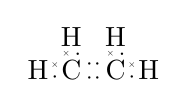
\begin{tikzpicture}[inner sep=0pt]
  \node (c1) at (-0.8em,0){\ce{C}};
  \node (c2) at (0.8em,0){\ce{C}};
  \node (h1) at (-0.8em,1.2em){\ce{H}};
  \node (h2) at (0.8em,1.2em){\ce{H}};
  \node (h3) at (-2.0em,0em){\ce{H}};
  \node (h4) at (2.0em,0em){\ce{H}};
  \draw [draw=none](c1)--(c2)
    node[pos=0.33,below=1pt]{\footnotesize$\cdot$}
    node[pos=0.33,above]{\footnotesize$\cdot$}
    node[pos=0.67,below=1pt]{\footnotesize$\cdot$}
    node[pos=0.67,above]{\footnotesize$\cdot$};
  \foreach \x/\y in {c1/h1,h3/c1,c2/h2,c2/h4}
  {
    \draw [draw=none](\x)--(\y)
      node[midway,sloped,above=0.5pt]{\scalebox{0.35}{$\times$}}
      node[midway,sloped,below=0.5pt]{\footnotesize$\cdot$};
  }
\end{tikzpicture}
\qquad\chemfig{H-C(-[:90]H)=C(-[:90]H)-H}\]

从乙烯的结构式可以看出，乙烯分子里含有 \ce{C=C} 双键，\emph{链烃分子里含有碳碳双键的不饱和烃叫做}\Concept{烯烃}。
乙烯是分子组成最简单的烯烃。

为了更简单形象地描述乙烯分子的结构，我们常用分子模型来表示（\cref{fig:2-7}）。在\cref{fig:2-7a} 的球棍模型里，两个碳原子间用两根可以弯曲的弹性短棍来连接，用它们来表示双键。\cref{fig:2-7b} 是乙烯分子的比例模型。
\begin{figure}
  \begin{minipage}[b]{0.48\linewidth}\centering
    \includegraphics{2-7a.pdf}
    \subcaption{球棍模型}\label{fig:2-7a}
  \end{minipage}
  \begin{minipage}[b]{0.48\linewidth}\centering
    \includegraphics{2-7b.pdf}
    \subcaption{比例模型}\label{fig:2-7b}
  \end{minipage}
  \caption{乙烯分子的模型}\label{fig:2-7}
\end{figure}

实验表明，乙烯分子里的 \ce{C=C} 双键的键长是 \qty{1.33e-10}{m}，乙烯分子里的两个碳原子和四个氢原子都处在同一平面上。
它们彼此之间的键角约为 \ang{120}。
乙烯双键的键能是 \qty{147}{kCal/mol}，实验测得乙烷 \ce{C-C} 单键的键长是 \qty{1.54e-10}{m}，键能是 \qty{83.1}{kCal/mol}。
这表明 \ce{C=C} 双键的键能并不是 \ce{C-C} 单键键能的两倍，而是比两倍略少。
因此，只需要较少的能量，就能使双键里的某一个键断裂。
这从下面介绍的乙烯的化学性质里可以得到证实。

\begin{Reading}[补充阅读]{}
乙烯分子为什么是这样的结构呢？

为了解释 \ce{CH2=CH2} 分子的平面形结构，杂化轨道理论认为碳原子的一个 $2s$ 轨道和两个 $2p$ 轨道进行了 $sp^2$ 杂化（\cref{fig:2-8a}），其余的一个 $p$ 轨道仍保持原状，没有参加杂化。

在构成乙烯分子时，两个碳原子各以 2 个 $sp^2$ 杂化轨道跟两个氢原子的 $1s$ 轨道进行重叠，形成 4 个碳氢的 $\sigma$ 键。
两个碳原子又各以一个 $sp^2$ 杂化轨道相互重叠，形成一个碳碳的 $\sigma$ 键。
分子里所有的 5 个 $\sigma$ 键都在同一平面上，键角约为 \ang{120}（\cref{fig:2-8b}）。
同时，每个碳原子还有一个未参加杂化的 $p$ 轨道，这两个 $p$ 轨道垂直于 5 个 $\sigma$ 键的对称轴所在的平面，并相互平行。
因此，这两个 $p$ 轨道可以在侧面重叠成键（\cref{fig:2-9}）。
这样形成的键叫做 $\pi$ 键。
它垂直于五个 $\sigma$ 键所处的平面。
\begin{figurehere}
  \begin{minipage}{0.3\linewidth}\centering
    \includegraphics{2-8a.pdf}
    \subcaption{}\label{fig:2-8a}
  \end{minipage}
  \begin{minipage}{0.66\linewidth}\centering
    \includegraphics{2-8b.pdf}
    \subcaption{}\label{fig:2-8b}
  \end{minipage}
\end{figurehere}
\begin{figurehere}
  \caption{乙烯分子里的 $\sigma$ 键}\label{fig:2-8}
\end{figurehere}

\begin{figurehere}
  \includegraphics{2-9.pdf}
  \caption{乙烯分子里的 $\pi$ 键}\label{fig:2-9}
\end{figurehere}

由此可见，乙烯分子里的 \ce{C=C} 双键是由一个 $\sigma$ 键和一个 $\pi$ 键形成的。
这两种键的轨道重叠程度是不同的。
$\pi$ 键是由 $p$ 轨道从侧面重叠形成的，重叠程度比 $\sigma$ 键从正面重叠要小，所以 $\pi$ 键不如 $\sigma$ 键牢固，比较容易断裂，断裂时需要的能量也较少。
同时，不象 $\sigma$ 键的电子云那样集中在连接两原子核的对称轴上，而是分散在上下两处。

由于碳原子核对 $\pi$ 键电子云的吸引力比较弱，因此 $\pi$ 键电子云在外界条件的影响下，易于变形。
这就是烯烃为什么较活泼，易于起加成等反应的原因。

已经知道 $\pi$ 键的形成是由于两个互相平行的 $p$ 轨道从侧面重叠的结果，如果这种平行的重叠受到破坏，就会导致 $\pi$ 键的断裂。
所以，双键跟单键不同，以双键相连接的碳原子是不能旋转的。
\end{Reading}

\subsection{乙烯的物理性质}
乙烯是没有颜色的气体，稍有气味，密度是 \qty{1.25}{g/L}，比空气略轻些，难溶于水。

\subsection{乙烯的化学性质和用途}
工业上所用的乙烯，是从石油炼制工厂和石油化工厂所生产的气体里分离出来的。
实验室里是把酒精和浓硫酸混和加热，使酒精分解制得。
浓硫酸在反应过程里起催化剂和脱水剂的作用。
% \[ \ce{ CH3-CH2-OH ->[\text{浓硫酸}][\qty{170}{\celsius}] CH2=CH2 ^ + H2O }\]
\[
\schemestart
\chemname{\chemfig{CH_3-CH_2-OH}}{乙醇}
\arrow(.mid east--.mid west){->[{\footnotesize 浓硫酸}][{\footnotesize \qty{170}{\celsius}}]} 
\chemname{\chemfig{CH_2=CH_2}}{乙烯} \ce{ ^ }
\+ \ce{H2O}
\schemestop\chemnameinit{}
\]
\begin{Experiment}*[righthand ratio=0.6]
把烧瓶和导管等装置如\cref{fig:2-10}。烧瓶里注入酒精和浓硫酸（体积比 $1:3$）的混和液约 \qty{20}{ml}，并放入几片碎瓷，以免混和液在受热沸腾时剧烈跳动。加热使液体温度迅速升到 \qty{170}{\celsius}，这时就有乙烯生成。
\tcblower 
\begin{figurehere}
  \includegraphics{2-10.pdf}
  \caption{乙烯的实验室制法}\label{fig:2-10}
\end{figurehere}
\end{Experiment}

\subsubsection{加成反应}
\begin{Experiment}
把乙烯通入盛溴水的试管里，可以观察到溴水的红棕色很快消失。
\end{Experiment}
乙烯能跟溴水里的溴起反应，生成无色的 1,2-二溴乙烷（\ce{CH2Br-CH2Br}）液体。
\[
\schemestart
\chemfig{H-C(-[:90]H)=C(-[:90]H)-H} \+ \chemfig{Br-Br}
\arrow(.mid east--.mid west)
\chemname{\chemfig{H-C(-[:90]H)(-[:-90]Br)-C(-[:90]H)(-[:-90]Br)-H}}{\footnotesize 1,2-二溴乙烷}
\schemestop\chemnameinit{}
\]

这个反应的实质是乙烯分子里的双键里的一个键易于断裂，两个溴原子分别加在两个价键不饱和的碳原子上，生成了二溴乙烷。
这种\emph{有机物分子里不饱和的碳原子跟其它原子或原子团直接结合生成别的物质的反应叫做}\Concept{加成反应}。

乙烯还能跟氢气、氯气、卤化氢以及水等在适宜的反应条件下起加成反应。
\begin{gather*}
  \ce{CH2=CH2 + H2 ->[\text{催化剂}] CH3-CH3} \\
  \ce{CH2=CH2 + HCl -> CH3-CH2Cl}
\end{gather*}

\subsubsection{氧化反应}
\begin{Experiment}
  点燃纯净的乙烯，它能在空气里燃烧，有明亮的火焰。同时发出黑烟。
\end{Experiment}
跟其它的烃一样，乙烯在空气里燃烧的时候，也生成二氧化碳和水。
但是乙烯分子里含碳量比较大，由于这些碳没有得到充分燃烧，所以有黑烟生成。
下面是乙烯完全燃烧的化学方程式。
\[ \ce{ CH2=CH2 + 3O2 ->[\text{点燃}] 2CO2 + 2H2O \text{（液）} } + \qty{337.2}{kCal} \]

乙烯不但能跟氧气直接发生氧化，并能被氧化剂所氧化。

\begin{Experiment}
  把乙烯通入盛有高锰酸钾溶液（加几滴稀硫酸）的试管里。可以观察到溶液的紫色很快褪去。
\end{Experiment}
乙烯可被氧化剂高锰酸钾（\ce{KMnO4}）氧化，使高锰酸钾溶液褪色。
用这种方法可以区别甲烷和乙烯。

\subsubsection{聚合反应}
在适当的温度、压强和有催化剂存在的条件下，乙烯分子里的双键会断裂其中的一个键，发生加成反应，使乙烯分子里的碳原子能够互相结合成为很长的链。
\begin{multline*} 
  \ce{ CH2=CH2 + CH2=CH2 + CH2=CH2 } \cdots\cdots \ce{ -> }\\
  \ce{-CH2-CH2- + -CH2-CH2- + -CH2-CH2- } \cdots\cdots \\
  \ce{ -> -CH2-CH2-CH2-CH2-CH2-CH2- } \cdots\cdots
\end{multline*}

这个反应还可以用下式表示：
\[ 
\schemestart
$n$\,\chemfig{CH_2=CH_2}
\arrow(.mid east--.mid west){->[\scriptsize 催化剂]}
\chemname{\chemfig{\vphantom{CH_2}-[@{op,.6}]CH_2-CH_2-[@{cl,0.4}]}\polymerdelim[delimiters ={[]},indice =\!n]{op}{cl}}{\footnotesize 聚乙烯}
\schemestop\chemnameinit{}
\]

反应的产物是聚乙烯。
它是一种式量很大（几万到几十万）的化合物，它的化学式可以简单地写为 \ce{(C2H4)_$n$}。
生成聚乙烯这样的反应属于聚合反应。
在这个聚合反应里，式量小的化合物分子互相结合为式量很大的化合物分子。
这样的聚合反应也是加成反应，所以又属于\Concept{加成聚合反应}，简称\Concept{加聚反应}。

从六十年代以来，世界上乙烯的产量飞速发展。
乙烯是石油化学工业最重要的基础原料，用于制造塑料、合成纤维、有机溶剂等。
乙烯的发展带动了其它石油化工基础原料和产品的发展。

乙烯还是一种植物生长调节剂，例如它可被用做果实催熟剂等。

\begin{Practice}[习题]
\begin{question}
  \item 怎样鉴别装在不同容器里的甲烷和乙烯？
  \item 在实验室里怎样从混有乙烯的甲烷里提纯甲烷？
  \item 当乙烯通过装有溴的试剂瓶的时候，试剂瓶的质量增加了 \qty{16}{g}。有多少升的乙烯（在标准状况下）被吸收了？生成了多少克的二溴乙烷？
  \item 乙烯跟氯化氢加成可以生成氯乙烷（\ce{C2H5Cl}），写出反应的化学方程式。按理论计算每吨乙烯能生产多少吨氯乙烷？
\end{question}
\end{Practice}

\section{烯烃}
\subsection{烯烃及其命名}
烯烃是分子里含有碳碳双键（\ce{C=C}）的不饱和链烃的总称。
烯烃里除乙烯外，还有丙烯（\ce{CH3CH=CH2}），丁烯（\ce{CH3CH2CH=CH2}）等等。\cref{tab:2-2} 列举几种乙烯的同系物的物理性质。
\begin{table}
  \caption{几种烯烃的物理性质}\label{tab:2-2}
  \begin{tblr}{colspec={cX[r]cS[table-format=5.2]S[table-format=5.2]l},hline{2}=0.8pt,row{1}={m,c,guard}}
    名称 & 结构简式 & {常温时\\状态} & 熔点 \unit{\celsius} & 沸点 \unit{\celsius} & {液态时的密度\\（\unit{g/cm^3}）}\\
    乙烯 & \ce{CH2=CH2}         & 气 & -169.2 & -103.7 & $0.384^*$ \\
    丙烯 & \ce{CH3CH=CH2}       & 气 & -185.3 & -47.4  & $0.5193$ \\
    丁烯 & \ce{CH3CH2CH=CH2}    & 气 & -185.4 & -6.3   & $0.5951$ \\
    戊烯 & \ce{CH3(CH2)2CH=CH2} & 液 & -138   & 29.97  & $0.6405$ \\
    己烯 & \ce{CH3(CH2)3CH=CH2} & 液 & -139.8 & 63.35  & $0.6731$ \\
    庚烯 & \ce{CH3(CH2)4CH=CH2} & 液 & -119   & 93.64  & $0.6970$ \\
  \end{tblr}\par
  \begin{minipage}{\linewidth}
    \footnotesize * 是 \qty{-10}{\celsius} 时的值，其余是 \qty{20}{\celsius} 时的值。
  \end{minipage}
\end{table}

由\cref{tab:2-2} 我们可以看出，跟烷烃一样，乙烯同系物也是依次相差一个 \ce{CH2} 原子团。
烯烃的通式是 \ce{C_$n$H_$2n$}。
它们的物理性质一般地也随着碳原子数目的增加而递变。
烯烃的化学性质也跟乙烯类似，如易于起加成反应等。

丙烯是石油工业的一种重要产品，也是一种重要的化工原料。
例如，通过加聚反应制造聚丙烯。

烯烃的命名跟烷烃类似，所不同的是要求表示出双键的位置。
命名的步骤是：
\begin{enumerate}[1.]
  \item 确定包括双键在内的碳原子数目最多的碳链为主链。
  \item 主链里碳原子的依次编号从离双键较近的一端算起。
  \item 双键的位置可以用阿拉伯数字标在某烯字样的前面。

  例如：
  \[ 
\schemestart
\chemname{\chemfig{CH_2=CHCH_2CH_3}}{\footnotesize 1-丁烯}\quad
\chemname{\chemfig{CH_3CH=CHCH_3}}{\footnotesize 2-丁烯}\quad
\chemname{\chemfig{CH_3-CH=CH-CH(-[:-90]CH_3)-CH_3}}{\footnotesize 4-甲基-2-丁烯}
\schemestop\chemnameinit{}
\]
  1-丁烯和 2-丁烯是同分异构体。
\end{enumerate}

\subsection{二烯烃}
分子里含有两个双键的链烃叫做二烯烃，如 1,3-丁二烯（\chemfig{\charge{90[anchor=-90]={\tiny 1}}{C}H_2=\charge{90[anchor=-90]={\tiny 2}}{C}H\charge{90[anchor=-90]={\tiny 3}}{C}H=\charge{90[anchor=-90]={\tiny 4}}{C}H_2}）就是二烯烃里的最重要的同系物。
1,3-丁二烯是一种重要的有机化工原料。

二烯烃有双键，也象烯烃一样能起加成反应等。
但是，1,3-丁二烯有两个双键，又有它的特点，在起加成反应时，两个双键里比较活泼的键能够一起断裂，而同时又生成一个新的双键。
例如，1,3-丁二烯跟 \ce{Br2} 进行的加成反应。
\[ \schemestart
\chemfig{\charge{90[anchor=-90]={\tiny 1}}{C}H_2=\charge{90[anchor=-90]={\tiny 2}}{C}H-\charge{90[anchor=-90]={\tiny 3}}{C}H=\charge{90[anchor=-90]={\tiny 4}}{C}H_2} \+ \ce{Br2} \arrow \chemfig{Br-\charge{90[anchor=-90]={\tiny 1}}{C}H_2-\charge{90[anchor=-90]={\tiny 2}}{C}H=\charge{90[anchor=-90]={\tiny 3}}{C}H-\charge{90[anchor=-90]={\tiny 4}}{C}H_2-Br}
\schemestop\chemnameinit{}\]
这种形式的加成反应叫 1,4-加成反应。

除生成这种 1,4 加成的产物外，还生成 1,2-加成产物：
\[ \chemfig{Br-\charge{90[anchor=-90]={\tiny 1}}{C}H_2-\charge{90[anchor=-90]={\tiny 2}}{C}HBr-\charge{90[anchor=-90]={\tiny 3}}{C}H=\charge{90[anchor=-90]={\tiny 4}}{C}H_2 } \]

在 1,3-丁二烯的加成反应里，1,4-加成产物通常是主要的。
1,4-加成反应在生产中有重要的意义。

二烯烃比烯烃多一个双键，少两个氢原子，所以二烯烃的通式是 \ce{C_$n$H_$2n-2$}。

\begin{Practice}
\begin{question}
  \item 写出式量是 56 的某链烃的各种同分异构体的结构式，并写出它们的名称。
  \item 写出\begin{enumerate*}\item 丙烯、\item 异丁烯\end{enumerate*}的电子式。
  \item 写出下列各烯烃的同分异构体的数目，并写出它们的结构式：
  \[\chemfig{CH_2=C(-[:-90]CH_3)-CH_3} \quad \chemfig{CH_3-CH=CH-CH_2-CH_3} \]
  \item 写出下列几种物质的结构简式：
  \begin{tasks}(3)
    \task  丙烯，
    \task  1-丁烯，
    \task  1,3-丁二烯，
    \task! 异戊二烯（即 2-甲基-1,3-丁二烯）。
  \end{tasks}
  \item 某种烃的化学式是 \ce{C5H10}，我们能不能说它一定是乙烯的同系物？为什么？
  \item 从环烷烃的化学式来看，它是哪一类链烃的同分异构体？
  \item 某烃 \qty{0.1}{mol} 完全燃烧后，生成 \qty{0.3}{mol} \ce{CO2} 和 \qty{0.3}{mol} \ce{H2O}，这种烃的化学式是什么？
\end{question}
\end{Practice}

\section[乙炔\ 炔烃]{乙炔\texorpdfstring{\protect\footnote{炔音\pinyin{que1}}\quad}{ }炔烃}
\subsection{乙炔的物理性质和结构式}
乙炔俗名电石气，纯的乙炔是没有颜色、没有臭味的气体，由电石制备的乙炔常因混有磷化氢、硫化氢等杂质而发出特殊难闻的臭味。
乙炔的密度是 \qty{1.16}{g/L}，比空气稍轻，微溶于水，易溶于有机溶剂。

乙炔的化学式是 \ce{C2H2}。从这个化学式可以看出，乙炔的分子比乙烯的分子少两个氢原子。
在乙炔分子里的碳原子间有三个共用电子对。
通常我们把它称为叁键，这可用下式表示：
\[ \quad \chemfig{H-C~C-H}\]

\cref{fig:2-11} 是乙炔分子的两种模型。
\begin{figure}
  \begin{minipage}[b]{0.48\linewidth}\centering
    \includegraphics{2-11a.pdf}
    \subcaption{球棍模型}\label{fig:2-11a}
  \end{minipage}
  \begin{minipage}[b]{0.48\linewidth}\centering
    \includegraphics{2-11b.pdf}
    \subcaption{比例模型}\label{fig:2-11b}
  \end{minipage}
  \caption{乙炔的分子模型}\label{fig:2-11}
\end{figure}

实验表明，乙炔分子里碳碳之间的叁键的键能是 \qty{194}{kCal/mol}，并不等于三个单键键能之和，比三个单键的键能要小得多（也比一个单键和一个双键键能之和小）。
叁键的键长是 \qty{1.20e-10}{m}，比单键和双键的键长都短。
并且已经证明乙炔分子里 \ce{C#C} 键跟 \ce{C-C} 键间的夹角是 \ang{180}，也就是说，乙炔分子里的两个碳原子和两个氢原子处在一条直线上。

\begin{Reading}[补充阅读]{}
乙炔分子为什么有这样的结构呢？
\begin{figurehere}
  \begin{minipage}[b]{0.4\linewidth}\centering
    \includegraphics{2-12a.pdf}
    \subcaption{$sp$ 杂化}\label{fig:2-12a}
  \end{minipage}
  \begin{minipage}[b]{0.58\linewidth}\centering
    \includegraphics{2-12b.pdf}
    \subcaption{$\sigma$ 键的形成}\label{fig:2-12b}
  \end{minipage}
  \caption{乙炔分子里 $\sigma$ 模型}\label{fig:2-12}
\end{figurehere}

杂化轨道理论对于乙炔分子结构的解释是，乙炔分子里每个碳原子在形成叁键时，是以一个 $2s$ 轨道和一个 $2p$ 轨道进行杂化，形成两个能量相等的沂轨道，叫做 $sp$ 杂化轨道（\cref{fig:2-12a}）。
这两个 $sp$ 杂化轨道的对称轴在同一条直线上。
每个碳原子各以一个 $sp$ 杂化轨道跟氢原子的一个 $1s$ 轨道进行重叠而形成一个碳氢的 $\sigma$ 键。
同时又各以其另一个 $sp$ 杂化轨道相互重叠形成一个碳碳的 $\sigma$ 键（\cref{fig:2-12b}）。
在两个碳原子里还各有另外两个 $p$ 轨道没有参加杂化，它们的电子云互相垂直，同时也跟碳碳间 $\sigma$ 键的对称轴垂直。
这样就在 4 个 $p$ 电子之间形成两个 $\pi$ 键,这两个 $\pi$ 键是互相垂直的（\cref{fig:2-13}）。

\begin{figurehere}
  \includegraphics{2-13.pdf}
  \caption{乙炔分子里 $\pi$ 键的形成}\label{fig:2-13}
\end{figurehere}

乙炔分子里的 \ce{C#C} 叁键是由一个 $\sigma$ 键和两个相互垂直的 $\pi$ 键所组成。
已知 $\pi$ 键键能小于 $\sigma$ 键键能，所以在一定条件下，$\pi$ 键容易断裂。
因此，具有叁键的化合物也很活泼，如易起氧化反应、加成反应等。
同时，叁键的键长也比双键更短一些。
\end{Reading}

\subsection{乙炔的制法、化学性质和用途}
\subsubsection{实验室制法}
乙炔在实验室里是用电石（碳化钙）跟水反应制得。
\[ \ce{ CaC2 + 2H2O -> C2H2 + Ca(OH)2} + \qty{30.33}{KCal} \]

\begin{Experiment}*[righthand ratio=0.5]\label{expr:2-9}
  实验装置如\cref{fig:2-14} 所示。在广口瓶里放几小块碳化钙。轻轻旋开分液漏斗的活栓，使水\footnote{碳化钙跟水的反应比较剧烈，为了得到平稳的乙炔气流，可以用包和食盐水代替水。食盐跟碳化钙不起反应。}缓慢地滴下。用排水法收集乙炔。观察乙炔的颜色、状态。
  \tcblower
  \begin{figurehere}
    \includegraphics{2-14.pdf}
    \caption{制取乙炔}\label{fig:2-14}
  \end{figurehere}
\end{Experiment}

\subsubsection{乙炔的化学性质}
\paragraph{氧化反应}\mbox{}\par
\begin{Experiment}
  点燃从\cref{expr:2-9} 制取的乙炔，观察火焰。
\end{Experiment}
乙炔完全燃烧的反应可以表示如下：
\[ \ce{ 2C2H2 + 5O2 ->[\text{点燃}] 4CO2 + 2H2O\,\text{（液）}} + \qty{621.2}{kCal}\]

乙炔燃烧时产生大量的热。
乙炔的成分里含碳量很大，所以燃烧不充分时发出光亮而带浓烟的火焰。乙炔跟空气的混和物遇火会发生爆炸\footnote{乙炔在空气里的爆炸极限是含乙炔 2.5\%～80\%。}，所以在生产和使用乙炔时,必须注意安全。
乙炔在氧气里燃烧时，产生的氧炔焰的温度很高（可达 \qty{3000}{\celsius} 以上），可以用来切割和焊接金属。
\begin{Experiment}
把纯净的乙炔通入盛有高锰酸钾溶液（加少量硫酸）的试管，观察紫色溶液的变化。
\end{Experiment}
乙炔也容易被氧化剂所氧化，能使高锰酸钾溶液的紫色褪去。

\paragraph{加成反应}\mbox{}\par
\begin{Experiment}
  把纯净的乙炔通入盛有溴水的试管，观察溶液颜色的变化。
\end{Experiment}
可以观察到乙炔也能使溴水褪色。反应过程可以分步表示如下：
\begin{gather*}
\schemestart
\chemfig{H-C~C-H} \+ \chemfig{Br-Br} \arrow(.mid east--.mid west)
\chemname{\chemfig{H-C(-[:-90]Br)=C(-[:-90]Br)-H}}{\footnotesize 1,2-二溴乙烯}
\schemestop\chemnameinit{}\\
\schemestart
\chemfig{H-C(-[:-90]Br)=C(-[:-90]Br)-H} \+ \chemfig{Br-Br} \arrow(.mid east--.mid west)
\chemname{\chemfig{H-C(-[:-90]Br)(-[:90]Br)-C(-[:-90]Br)(-[:90]Br)-H}}{\footnotesize 1,1,2,2-四溴乙烷}
\schemestop\chemnameinit{}
\end{gather*}

如果用镍粉作催化剂并且加热，乙炔就能跟氢气进行加成反应，先生成乙烯，再成为乙烷。
\begin{gather*}
  \ce{   CH#CH + H2 ->[\text{催化剂}][\triangle] CH2=CH2} \\
  \ce{ CH2=CH2 + H2 ->[\text{催化剂}][\triangle] CH3-CH3} 
\end{gather*}

乙炔跟溴、氢气的加成反应，有力地证明了乙炔结构式的正确性。

在 \qtyrange{150}{160}{\celsius} 和氯化汞作为催化剂的条件下，乙炔能跟氯化氢进行加成反应，生成氯乙烯。
氯乙烯是重要的化工原料。
% \[ \ce{ HC#CH + HCl ->[\text{催化剂}][\triangle] CH2=CHCl } \]
\[\schemestart
\chemfig{HC~CH} \+ \chemfig{HCl} 
\arrow(.mid east--.mid west){->[\footnotesize 催化剂][\footnotesize $\triangle$]}
\chemname{\chemfig{CH_2=CHCl}}{\footnotesize 氯乙烯}
\schemestop\chemnameinit{}\]

\subsubsection{乙炔的用途}
从乙炔的性质可以知道，由乙炔开始能制出氯乙烯等许多重要有机化学工业的原料，所以乙炔是一种重要的基本有机原料。
但是，从电石生产乙炔，需要消耗大量的电，所以今后趋向于用天然气和石油作为原料来生产乙炔。

\subsection{炔烃}
\emph{链烃分子里含有碳碳叁键的不饱和烃叫做}\Concept{炔烃}。
除乙炔外还有丙炔、丁炔等等。
\cref{tab:2-3} 是几种乙炔同系物的名称、结构简式和物理性质。
\begin{table}
  \caption{几种块烃的物理性质}\label{tab:2-3}
  \begin{tblr}{colspec={cX[r]cS[table-format=5.2]S[table-format=5.2]l},hline{2}=0.8pt,row{1}={m,c,guard}}
    名称 & 结构简式 & {常温时\\状态} & 熔点 \unit{\celsius} & 沸点 \unit{\celsius} & {液态时的密度\\（\unit{g/cm^3}）}\\
    乙炔   & \ce{H-C#CH}           & 气 & -80.8 & -84.0 & $0.6181^*$ \\
    丙炔   & \ce{CH3-C#CH}        & 气 & -101.5 & -23.2 & $0.66^{**}$ \\
    1-丁炔 & \ce{CH3-CH2-C#CH}    & 气 & -125.7 & 8.1 & $0.6784^{***}$ \\
    1-戊炔 & \ce{CH3-(CH2)2-C#CH} & 液 & -90 & 40.18 & $0.6901$ \\
  \end{tblr}\par
  \begin{minipage}{\linewidth}
    \footnotesize * 是 \qty{-32}{\celsius} 时的值，** 是 \qty{-13}{\celsius} 时的值，*** 是 \qty{0}{\celsius} 时的值，另一是 \qty{20}{\celsius} 时的值。
  \end{minipage}
\end{table}

从\cref{tab:2-3} 可知，乙炔的各同系物也依次相差一个 \ce{CH2} 原子团，但它们比同级的烯烃各少两个氢原子，所以炔烃的通式是 \ce{C_$n$H_$2n-2$}。
炔烃的物理性质一般也是随着分子里碳原子数的增多而递变的。

\begin{Practice}[习题]
\begin{question}
  \item 使 \qty{13}{g} 乙炔完全燃烧，在 \qty{1}{atm} 和 \qty{27}{\celsius} 时需要用多少升空气？
  \item 比较乙烷、乙烯、乙炔的化学性质。
  \item 相同摩尔数的乙烷、乙烯和乙炔完全燃烧后生成的二氧化碳和水的量是不是相等？产生的热量是不是相等？用热化学方程式来说明。
  \item 指出下列化学式各代表哪类直链烃：
  \begin{tasks}(5)
    \task \ce{C8H16}，
    \task \ce{C9H16}，
    \task \ce{C15H32}，
    \task \ce{C17H34}，
    \task \ce{C7H12}。
  \end{tasks}
  \item 哪类烃叫做不饱和链烃？你所知道的不饱和链烃可以分成哪几类？不饱和链烃具有哪些特性？
  \item 在标准状况下，\qty{11.2}{L} 乙炔跟溴起加成反应，需要溴的最大数量是多少克？
  \item 含杂质 10\% 的碳化钙 \qty{100}{g}，在 \qty{25}{\celsius} 和 \qty{770}{mmHg} 时能够制得乙炔多少升？
  \item 通式为 \ce{C_$n$H_$2n-2$} 的一种炔烃完全燃烧后，生成的 \ce{CO2} 和 \ce{H2O} 的摩尔数比是 $2:1$，写出这种炔烃的化学式。
\end{question}
\end{Practice}

\section[苯\  芳香烃]{苯\texorpdfstring{\protect\footnote{苯音\pinyin{ben3}}\quad}{ }芳香烃}
\subsection{苯分子的结构}
苯是没有颜色带有特殊气味的液体，比水轻，不溶于水。
苯的沸点是 \qty{80.1}{\celsius}，熔点是 \qty{5.5}{\celsius}。
如果用冰来冷却，苯可以凝结成无色的晶体。

苯的化学式是 \ce{C6H6}。
从苯的化学式看，苯是远没有达到饱和的烃。
因为苯的分子需要增加 8 个氢原子才符合饱和链烃的通式： \ce{C_$n$H_$2n+2$}。
根据长期研究，认为苯的结构式可以这样表示：
\[
\chemfig{C*6(=C(-[:-90]H)-C(-[:0]H)=C(-[:0]H)-C(-[:90]H)=C(-[:180]H)-)(-[:180]H)}
\quad \text{或者简写为}\ \chemfig{*6(=-=-=-)} \]

从这样的结构式（又称凯库勒式）来推测，苯的化学性质应该显示出不饱和烃的性质。
是不是这样呢？让我们仔细观察下面的实验。
\begin{Experiment}
在盛有苯的两个试管里，分别加入高锰酸钾的酸性溶液和溴水，结果溶液颜色都保持不变。这说明苯跟高锰酸钾溶液或溴水都不起反应。
\end{Experiment}

由此可知，苯跟一般烯烃在性质上有很大区别。

对苯的结构作进一步的研究后知道，苯分子具有平面的正六边形结构。
各个键角都是 \ang{120}，六角环上碳碳之间的键长都是 \qty{1.40e-10}{m}。
它既不同于一般的单键（\ce{C-C} 键键长是 \qty{1.54e-10}{m}），也不同于一般的双键（\ce{C=C} 键键长是 \qty{1.33e-10}{m}）。

从苯跟高锰酸钾溶液和溴水都不起反应这一事实和测定的碳碳间键长的实验数据来看，充分说明苯环上碳碳间的键应是一种介于单键和双键之间的独特的键。
为了表示苯分子结构这一特点，常用右式来表示苯的结构简式 \chemfig[atom sep=0.5em]{[:30]**6(------)}。

苯分子模型可以如\cref{fig:2-15} 那样表示：
\begin{figure}
  \includegraphics{2-15.pdf}
  \caption{苯分子模型}\label{fig:2-15}
\end{figure}

直到现在，凯库勒式的表示方法仍被沿用，但在使用时绝不应认为苯是单、双键交替组成的环状结构。

在有机化合物里有一大类化合物叫做芳香族化合物\footnote{在已知的芳香族化合物里，大都是没有香味的。现在芳香族化合物这个名称已失去了它原来的意义（历史上是指一类从植物胶里取得的具有芳香气味的物质），只是因为使用这个名词已经习惯了，所以沿用到现在。}。\emph{分子里含有一个或多个苯环的化合物属于芳香族化合物}。
因此，我们可以说，苯环是芳香族化合物的母体。
苯是最简单、最基本的芳烃。

\begin{Reading}[补充阅读]{}
苯分子为什么是这样的结构呢？

按照杂化轨道理论，苯分子里六个碳原子的电子都以 $sp^2$ 杂化轨道相互重叠，形成六个碳碳的 $\sigma$ 键，又各以一个 $sp^2$ 杂化轨道分别跟氢原子的 \({1s}\) 轨道进行重叠，形成 6 个碳氢的 $\sigma$ 键。
由于是 $sp^2$ 杂化，所以键角是 \ang{120}，并且所有 6 个碳原子和 6 个氢原子都是在同一平面上相互连接起来的（\cref{fig:2-16}）。苯环上六个碳原子各有一个未参加杂化的 $2p$ 轨道，它们垂直于环的平面，并从侧面相互重叠而形成一个闭合的 $\pi$ 键（\cref{fig:2-17}），
\begin{figurehere}
  \nextfloat
  \begin{minipage}[b]{0.48\linewidth}\centering
    \includegraphics{2-16a.pdf}
    \subcaption{轨道重叠成 $\sigma$ 键}\label{fig:2-16a}
  \end{minipage}
  \begin{minipage}[b]{0.48\linewidth}\centering
    \includegraphics{2-16b.pdf}
    \subcaption{$\sigma$ 键分布示意图}\label{fig:2-16b}
  \end{minipage}
  \caption{苯分子内 $\sigma$ 键形成示意图}\label{fig:2-16}
\end{figurehere}
并且均匀地对称分布在环平面的上方和下方。
通常把苯的这种键型称为大 $\pi$ 键。
苯的大 $\pi$ 键的形成使 $\pi$ 键电子云不是只为某两个碳原子所共用，而是为 6 个碳原子所共用，因而受到六个碳原子核的共同吸引，彼此结合得比较牢固。
所以苯的性质比不饱和烃稳定，如在通常情况下不易发生一般不饱和烃所容易发生的加成反应等。
同时，苯的大 $\pi$ 键是平均分布在六个碳原子上，所以苯分子中每个碳碳键的键长和键能是相等的。
\begin{figurehere}
  \nextfloat
  \begin{minipage}[b]{0.48\linewidth}\centering
    \includegraphics{2-17a.pdf}
    \subcaption{$p$ 轨道重叠}\label{fig:2-17a}
  \end{minipage}
  \begin{minipage}[b]{0.48\linewidth}\centering
    \includegraphics{2-17b.pdf}
    \subcaption{大 $\pi$ 键的形成}\label{fig:2-17b}
  \end{minipage}
  \caption{苯分子大 $\pi$ 键的形成}\label{fig:2-17}
\end{figurehere}
\end{Reading}

\subsection{苯的化学性质和用途}
\subsubsection{取代反应}
苯分子里的氢原子能分别被别的原子或原子团所取代。

\paragraph{苯跟卤素的取代反应}\mbox{}\par
\begin{Experiment}*[righthand ratio=0.4]
把苯和少量液态溴放在烧瓶里，同时加入少量铁屑作催化剂\footnote{实际上起催化作用的是铁跟溴反应生成的溴化铁（\ce{FeBr3}）。}。用带导管的瓶塞塞紧瓶口（\cref{fig:2-18}），跟瓶口垂直的一段导管可以兼起冷凝器的作用。在常温时，很快就会看到，在导管口附近出现白雾（由溴化氢遇水蒸气所形成）。反应完毕后,向锥形瓶里的液体里滴入 \ce{AgNO3} 溶液，有浅黄色溴化银沉淀生成。把烧瓶里的液体倒在盛有冷水的烧杯里，烧杯底部有褐色不溶于水的液体。
\tcblower
\begin{figurehere}
  \includegraphics{2-18.pdf}
  \caption{苯跟溴的取代反应}\label{fig:2-18}
\end{figurehere}
\end{Experiment}
不溶于水的液体是溴苯，它是比水重的无色液体，由于溶解了溴而显褐色。苯跟溴的取代反应可以用化学方程式表示如下：
\[
\schemestart
\chemfig{[:-30]*6(=-=-=-)} \+ \chemfig{Br_2}
\arrow(.mid east--.mid west){->[\footnotesize 催化剂]}
\chemname{\chemfig{[:-30]*6(=-=(-Br)-=-)}}{\footnotesize 溴苯}
\+ \chemfig{HBr}
\schemestop\chemnameinit{}
\]

在催化剂作用下，苯也能跟其它卤素起取代反应。

\paragraph{苯的硝化反应}\mbox{}\par
\begin{Experiment}
在一个大试管里，先加入 \qty{1.5}{ml} 浓硝酸和 \qty{2}{ml} 浓硫酸，摇匀，冷却到 \qtyrange{50}{60}{\celsius} 以下，然后慢慢地滴入 \qty{1}{ml} 苯，不断摇动，使混和均匀，然后放在 \qty{60}{ \celsius} 的水浴中加热 \qty{10}{min}，把混和物倒入另一个盛水的试管里。可以明显地看到，有一种油状物生成。
\end{Experiment}

这种油状液体是硝基苯 \ce{C6H5NO2}，反应的化学方程式可以表示如下：
\[
\schemestart
\chemfig{[:-30]*6(=-=-=-)} \+ \chemfig{HO-NO_2}
\arrow(.mid east--.mid west){->[\footnotesize 催化剂][\footnotesize $\triangle$]}
\chemname{\chemfig{[:-30]*6(=-=(-NO_2)-=-)}}{\footnotesize 硝基苯}
\+ \chemfig{H_2O}
\schemestop\chemnameinit{}
\]

苯分子里的氢原子被 \ce{-NO2} 所取代的反应，叫做\Concept{硝化反应}。
硝酸分子里的 \ce{-NO2} 原子团叫做\Concept{硝基}。

硝基苯是一种没有颜色的油状液体，不纯的显淡黄色。
硝基苯有苦杏仁气味，比水重，有毒，是制造染料的重要原料。

\paragraph{苯的磺化反应}\mbox{}\par
共热到 \qtyrange{70}{80}{\celsius}，苯跟浓硫酸起反应。
在这个反应里，苯分子里的氢原子被硫酸分子里的\Concept{磺酸基}（\ce{-SO3H}）所取代而生成苯磺酸（\ce{C6H5-SO3H}）。这种反应叫做\Concept{磺化反应}。
\[
\schemestart
\chemfig{[:-30]*6(=-=-=-)} \+ \chemfig{HO-SO_3H}
\arrow(.mid east--.mid west){->[\footnotesize $\triangle$]}
\chemname{\chemfig{[:-30]*6(=-=(-SO_3H)-=-)}}{\footnotesize 苯磺酸}
\+ \chemfig{H_2O}
\schemestop\chemnameinit{} 
\]

苯的硝化反应和磺化反应都属于取代反应。

\subsubsection{加成反应}
苯不具有典型的双键所应有的加成反应性能，但在特殊情况下，它仍能够起加成反应。
如有镍催化剂存在和在 \qtyrange{180}{250}{\celsius} 的条件下，苯可以跟氢起加成反应，即生成饱和环烃。
\[
\schemestart
\chemfig{*6(-=-=-=)} \+ \chemfig{3H_2}
\arrow(.mid east--.mid west){->[\footnotesize 催化剂][\footnotesize $\triangle$]}
\chemname{\chemfig{H_2C*6(-C(-[:-90,0.5,,,line width=0pt]H_2)-CH_2-CH_2-C(-[:90,0.5,,,line width=0pt]H_2)-C(-[:180,0.5,,,line width=0pt]H_2)-)}}{\footnotesize 环己烷}
\schemestop\chemnameinit{}
\]

在光照条件下，苯跟氯气起加成反应，生成六氯环己烷（\ce{C6H6Cl6}），它曾是一种使用较广的农药，即六六六，有杀虫作用。
但由于它的化学性质稳定，能在动植物体内和环境中累积，容易污染环境和食物。
因此，对六六六采取了限制使用和用高效、低毒、低残留的新品种农药取代的措施。

\subsubsection{苯在空气里燃烧}
苯在空气里能燃烧生成二氧化碳和水，燃烧时发生明亮并带有浓烟的火焰，这由于苯分子里含碳量很大的缘故。

苯是一种很重要的有机化工原料，它广泛用来生产合成纤维、合成橡胶、塑料、农药、医药、染料、香料等。
苯也常用作有机溶剂。

在从前，苯是从炼焦所得的煤焦油里提取的，产量受到一定的限制。
自从石油工业迅速发展以来，大量的苯可以从石油工业获得。

\medskip
\begin{Theorem}{讨论}
比较苯跟甲烷、乙烯的化学性质，你对苯跟烷烃和烯烃的性质既相似又不相似的事实怎样理解？
\end{Theorem}

\subsection{苯的同系物}
甲苯 \ce{C7H8}、二甲苯 \ce{C8H10} 等化合物的分子里都含有一个苯环结构。
它们都是苯的同系物。
苯的同系物的通式是 \ce{C_$n$H_$2n-6$}（$n\geqslant6$）。
它们都是芳香烃。
苯分子里的一个氢原子被甲基 \chemfig{CH_3-} 取代后生成甲苯 \chemfig[atom sep=0.7em]{[:30]*6(=-(-[:0,2]CH_3)=-=-)}。
两个氢原子被两个甲基取代后生成二甲苯。
由于取代位置不同，二甲苯有下列三种异构体：
\[\schemestart 
\chemname{\chemfig{[:-30]*6(-=-=(-[:90]CH_3)-(-[:90]CH_3)=)}}{\footnotesize 邻-二甲苯\\（沸点：\qty{144.4}{\celsius}）}\qquad\qquad
\chemname{\chemfig{CH_3-*6(-=-=(-[:90]CH_3)-=)}}{\footnotesize 间-二甲苯\\（沸点：\qty{139.1}{\celsius}）}\qquad
\chemname{\chemfig{CH_3-*6(-=-(-CH_3)=-=)}}{\footnotesize 对-二甲苯\\（沸点：\qty{138.4}{\celsius}）}
\schemestop\chemnameinit{}\]

苯的同系物在性质上跟苯有许多和似之处，如燃烧时都发生带有浓烟的火焰，也都能起取代反应等。

由于苯环和侧链的相互影响，使苯的同系物也有一些化学性质跟苯不同。
\begin{Experiment}
把甲苯、二甲苯各 \qty{2}{ml} 分别注入两个试管，各加入高锰酸钾酸性溶液 3 滴，用力振荡，结果紫色褪去。
\end{Experiment}
这一实验说明，甲苯、二甲苯能被高锰酸钾氧化，但被氧化的是苯环上的侧链，即甲基。

我们已经学过链烃、环烃和芳烃，为了区别于成环的环烷烃、芳烃等，链烃又叫脂肪烃。
脂肪烃因跟脂肪类物质有类似结构而得名。

\subsection[萘和蒽]{萘和蒽\texorpdfstring{\protect\footnote{萘音\pinyin{nai4},蒽音\pinyin{en1}}}{}}
在煤焦油里除了可以提取苯及其同系物外，还可以提取萘和蒽等其它芳香烃。
\subsubsection{萘（\ce{C10H8}）}
萘是一种重要的化工原料，它的结构式是：
\[ \chemfig{C*6(=C(-[:-90]H)-C(*6(-C(-[:-90]H)=C(-[:0]H)-C(-[:0]H)=C(-[:90]H)-#(,6pt)))=C-C(-[:90]H)=C(-[:180]H)-)(-[:180]H)} \quad \text{或简写成}\quad \chemfig{*6(=-(*6(-=-=-))=-=-)}\]

萘是一种无色片状的晶体，熔点为 \qty{80.55}{\celsius}，具有特殊的气味。
它不溶于水，易升华。
萘可以用来杀菌、防蛀、驱虫。
日常用的卫生球的主要成分就是萘。

\subsubsection{蒽（\ce{C14H10}）}
蒽也是一种重要的化工原料，它的结构式是：
\[ \chemfig{C*6(=C(-[:-90]H)-C(*6(C-C(-[:-90]H)=C(*6(-C(-[:-90]H)=C(-[:0]H)-C(-[:0]H)=C(-[:90]H)-#(,6pt)))-C=C(-[:90]H)-#(,6pt)))=C-C(-[:90]H)=C(-[:180]H)-)(-[:180]H)} \ \text{或简写成}\ \chemfig{*6(=-(*6(-=(*6(-=-=-))-=-))=-=-)} \]

蒽也是一种无色的晶体，熔点为 \qty{216.2}{\celsius}，易升华。
蒽是生产染料的重要原料。

萘和蒽都是由两个或两个以上的苯环分别共用相邻的碳原子而成的芳香烃。
这种芳香烃特称为稠环芳香烃。

\begin{Practice}[习题]
\begin{question}
  \item 怎样通过实验来区别苯、己烷和己烯？
  \item 某烃的化学式是 \ce{C8H10}，它不能使溴水褪色，但能使高锰酸钾酸性溶液褪色，能跟氢起加成反应，生成乙基环己烷。写出这种烃的结构式。
  \item 下列各种化合物各属于哪一类烃？写出它们的名称和结构式：
  \begin{tasks}(4)
    \task \ce{C6H5-C3H7}，
    \task \ce{C6H14}，
    \task \ce{C6H6}，
    \task \ce{C3H6}，
    \task \ce{C2H2}，
    \task*(2) \ce{CH3-CH2-CH=CH2}，
    \task \ce{C3H4}，
    \task \ce{C10H8}。
  \end{tasks}
\end{question}
\end{Practice}

\section{石油和石油产品概述}
烃的自然界来源主要是石油和天然气。
天然气的主要成分是甲烷，它含甲烷可达 80\%～98\%（体积百分比）。
有的天然气还含有乙烷、丙烷，以及 \ce{CO2}、\ce{N2} 等等，常因产地的不同，成分也有差别。
天然气是一种优良的气体燃料。

石油是一种极其重要的资源，是发展国民经济和国防建设的重要物资。
通过石油炼制，可以得到汽油、煤油、柴油等燃料和各种机器所需要的润滑油以及许多气态烃（称为炼厂气）等产品。
用石油产品和石油气（炼厂气、油田气、天然气）做原料来生产化工产品的工业简称石油化工。
利用石油产品做原料，通过化工过程，可以制造合成纤维、合成橡胶、塑料以及农药、化肥、炸药、医药、染料、油漆、合成洗涤剂等产品。
石油产品已被广泛地应用到国民经济各个部门。
所以人们把石油称为“工业的血液”。

\subsection{石油的成分}
石油是由古代动植物遗体经过非常复杂的变化而形成的一种粘稠状液体。
石油通常显黑色或深棕色，常有绿色或蓝色荧光，有特殊的气味，不溶于水，比水稍轻；没有固定的熔点和沸点。

石油所含的基本元素是碳和氢。
两种元素的总含量平均为 97\%～98\%，也有达到 99\% 的；同时还含有少量的硫、氧、氮等。石油的化学成分随产地不同而不同。
石油主要是由各种烷烃、环烷烃和芳香烃所组成的混和物。
石油的大部分是液态烃，同时在液态烃里溶有气态烃和固态烃。

\subsection{石油的炼制}
从油田里开采出来没有经过加工处理的石油叫原油。
原油成分复杂，还含有水和氯化钙、氯化镁等盐类。
含水多，在炼制时要浪费燃料；含盐多会腐蚀设备。
所以原油必须先经过脱水、脱盐等处理过程，才能进行炼制。
\subsubsection{石油的分馏}
经过脱水、脱盐的石油主要是烃类的混和物，因此没有固定的沸点。
在烃分子里，一般是含碳原子数越少的，沸点越低；含碳原子数越多的，沸点越高。
因此给石油加热时，低沸点的烃先气化，经过冷凝先分离出来。
随着温度升高，较高沸点的烃再气化，经过冷凝也分离出来。
这样继续加热和冷凝，就可以把石油分成不同沸点范围的蒸馏产物。
这种方法叫做石油的分馏。
分馏出来的各种成分叫馏分（每一种馏分仍然是多种烃的混和物）。
\begin{Experiment}
如\cref{fig:2-19} 装置，先认真检查装置是否气密之后，把 \qty{100}{ml} 原油注入蒸馏烧瓶，再加入几片碎瓷片（以防液体暴沸），然后给烧瓶加热，分别收集沸点为 \qtyrange{60}{150}{\celsius} 和 \qtyrange{150}{300}{\celsius} 的馏分。这样就得到汽油和煤油。
\tcblower
\begin{figurehere}
  \includegraphics{2-19.pdf}
  \caption{实验室蒸馏石油}\label{fig:2-19}
\end{figurehere}
\end{Experiment}
在炼油厂里分馏石油，原理跟上述实验一样，只是设备大，精密度高，能进行连续生产等。
工业上用来分馏石油的设备主要有: 加热炉，用于加热原油；分馏塔，利用原油里各成分沸点不同，分馏出各种产品。

分馏的主要过程（\cref{fig:2-20}）是把处理过的原油压入加热炉，加热到 \qty{360}{\celsius} 左右，使原油成为液体和气体的混和物，从导管进入分馏塔。
在分馏塔里，按各种烃的沸点不同（也就是挥发性大小的不同），在不同层的塔盘上分离出重油、柴油、煤油等。
沸点最低的烃以蒸气状态从分馏塔顶出来以后，再经冷凝成汽油（其中包括溶剂油）。
\begin{figure}
  \includegraphics{2-20.pdf}
  \caption{石油分馏示意图}\label{fig:2-20}
\end{figure}

从分馏塔底流出的重油可以再加以分离。
如果在常压下要分离重油里的物质，就必须再升高温度。
但是，在高温下，高沸点的烃受热会分解，更严重的是还会出现炭化结焦，损坏设备，影响正常生产。
为了解决这一矛盾，在石油炼制工业上常采用减压分馏的方法。
减压分馏的原理是利用外界压强对物质沸点的影响，因为外界压强越大，物质的沸点就越高；外界压强越小，物质的沸点就越低。
用降低分馏塔内压强的办法，能使重油的沸腾温度随压强降低而降低。
也就是说，在低于常压下的沸腾温度时就可以使重油沸腾，这种过程就是减压分馏。
为了区别起见，人们把在通常压强下的分馏叫做常压分馏。
在减压分馏塔里，仍根据沸腾温度范围的不同，从塔顶和塔的各种不同高度分离出重柴油以及各种不同规格的润滑油馏分等。
塔底出来的是渣油。

润滑油馏分还要进行加工，脱去凡士林、石蜡等，再经精制才能得到各种润滑油。
渣油经过处理，可以制造沥青，或进行焦化以制取石油焦。

现代炼油厂一般都把常压分馏塔和减压分馏塔装置在一起，所以习惯上称它作常、减压分馏。

石油分馏的产品和它们的用途见\cref{tab:2-4}。
\begin{table}
  \caption{石油分馏的产品和用途}\label{tab:2-4}
  \begin{tblr}{colspec={cX[c]X[c]cX[2,l]},hline{2}=0.8pt,row{1}={m,c}}
    \SetCell[c=2]{m,c} 分馏产品& & 分子所含碳原子数& 沸点范围 & 用途 \\
    \SetCell[c=2]{m,c} 溶剂油 & & \ce{C5}～\ce{C6} & \qtyrange{30}{150}{\celsius} & 在油脂、橡胶、油漆生产中作溶剂\\
    \SetCell[c=2]{m,c} 汽油 & & \ce{C5}～\ce{C11} & \qty{220}{\celsius} 以下 & 飞机、汽车以及各种汽油机燃料\\
    \SetCell[c=2]{m,c} 航空煤油 & & \ce{C10}～\ce{C15} & \qtyrange{150}{250}{\celsius} & 喷气式飞机燃料\\
    \SetCell[c=2]{m,c} 煤油 & & \ce{C11}～\ce{C16} & \qtyrange{180}{310}{\celsius} & 拖拉机用燃料、工业洗涤剂\\
    \SetCell[c=2]{m,c} 柴油 & & \ce{C15}～\ce{C18} & \qtyrange{200}{360}{\celsius} & 重型汽车、军舰、轮船、坦克、拖拉机、各种高速柴油机燃料\\
    \SetCell[r=5]{m,c} {重\\油}
    & 润滑油（锭子油、机油、汽缸油等）& \ce{C18}～\ce{C20} & \SetCell[r=5]{m,c} \qty{360}{\celsius} 以上 & 机械上的润滑剂、减少机械磨损、防锈 \\
    & 凡士林 & 液态烃和固态烃的混合物 & & 润滑剂、防锈剂、制药膏 \\
    & 石蜡   & \ce{C20}～\ce{C30} & & 制蜡纸、绝缘材料 \\
    & 沥青   & \ce{C30}～\ce{C40} & & 铺路，建筑材料，防腐涂剂 \\
    & 石油焦 & 主要成分是 \ce{C} & & 制电极，生产 \ce{SiC} 等 \\
  \end{tblr}\par
  \begin{minipage}{\linewidth}
    \footnotesize 注：表内所示沸点范围不是绝对的，在生产时常需根据具体情况进行一些变动。
  \end{minipage}
\end{table}

汽油是重要的燃料，广泛地应用于交通和国防建设的各个方面。
汽油质量的高低，对于使用有很大的关系。
那么汽油的质量是按什么标准来衡量的呢？
从石油经过直接分馏的方法得到的汽油（通常叫它直馏汽油）在使用时爆震性很强，会发出很大的噪声，降低汽油机的效率，消耗能量，因此不利于作燃料。
这就要求生产爆震性较小的汽油。

\begin{Reading}[补充阅读]{}
人们把抗震性能作为衡量汽油质量高低的一种标准。
通常是用“辛烷值”的大小来衡量汽油的抗震性能的。
辛烷值越大，汽油的抗震性能越好。
为什么叫做“辛烷值”呢？
原来有一种叫做异辛烷（2,2,4-三甲基戊烷）的化合物，
\[\schemestart 
\chemname{\chemfig{CH_3-CH(-[:-90]CH_3)-CH_2-C(-[:90]CH_3)(-[:-90]CH_3)-CH_3}}{\footnotesize 异辛烷（2,2,4-三甲基戊烷）}
\schemestop\chemnameinit{} \]
它的爆震性最弱，人们规定它的抗震性为 100；另外选择一种爆震性极强的正庚烷（\ce{C7H16}），规定它的抗震性为 0。
把汽油样品的抗震性跟这两种烃的不同成分的混和液的抗震性进行比较，就可以得出该汽油的辛烷值。
例如，经测定，一种汽油的抗震性跟含 66\% 的异辛烷和 34\% 的正庚烷的混和液的抗震性相等，那么，这种汽油的辛烷值就是 66。

为了提高汽油的抗震性能，通常还可以在汽油里加入少量抗震剂。
这样，就可以提高汽油的辛烷值。
\end{Reading}

为了更多地从石油里得到较高质量的汽油等产品，可对石油进行裂化、重整等加工方法。

\subsubsection{裂化}
石油通过分馏的方法获得汽油、煤油和柴油等轻质液体燃料。
但产量不高，仅占石油总量的 25\% 左右。
为了提高轻质液体燃料的产量，特别是提高汽油的产量，在石油工业上采用了裂化的方法。
裂化就是在一定条件下，把式量大、沸点高的烃断裂为式量小、沸点低的烃的过程。
裂化有热裂化和催化裂化。

重油、石蜡等含较大的烃分子，在 \qty{500}{\celsius} 左右和一定的压强下，被裂化而转变为式量较小的烃。
例如\footnote{这里所举的是简单的例子，实际上石油裂化的反应过程是很复杂的，同一种烃在裂化过程里可以起不同的分解反应。}：
\[\schemestart 
\chemname{\ce{C16H34}}{\footnotesize 十六烷}
\arrow(.mid east--.mid west){->[\footnotesize $\triangle$]}
\chemname{\ce{C8H18}}{\footnotesize 辛烷}
\+
\chemname{\ce{C8H16}}{\footnotesize 辛烯}
\schemestop\chemnameinit{}\]
这样就生成了式量比较小、沸点比较低的、类似汽油的饱和烃和不饱和烃的液态混和物。

有些裂化产物还会继续分解，生成饱和的和不饱和的气态烃。例如：
% \begin{gather*}
\[\schemestart 
\chemname{\ce{C8H18}}{\footnotesize 辛烷}
\arrow(.mid east--.mid west){->[\footnotesize $\triangle$]}
\chemname{\ce{C4H10}}{\footnotesize 丁烷}
\+
\chemname{\ce{C4H8}}{\footnotesize 丁烯}\\
\schemestop\chemnameinit{}\]
\[\schemestart 
\chemname{\ce{C4H10}}{\footnotesize 丁烷}
\arrow(.mid east--.mid west){->[\footnotesize $\triangle$]}
\chemname{\ce{CH4}}{\footnotesize 甲烷}
\+
\chemname{\ce{C3H6}}{\footnotesize 丙烯}
\schemestop\chemnameinit{}\]
\[\schemestart 
\chemname{\ce{C4H10}}{\footnotesize 丁烷}
\arrow(.mid east--.mid west){->[\footnotesize $\triangle$]}
\chemname{\ce{C2H6}}{\footnotesize 乙烷}
\+
\chemname{\ce{C2H4}}{\footnotesize 乙烯}
\schemestop\chemnameinit{}\]
  % \ce{ C8H18 ->[\triangle] C4H10 + C4H8 } \\
  % \ce{ C4H10 ->[\triangle] CH4 + C3H6 } \\
  % \ce{ C4H10 ->[\triangle] C2H4 + C2H6 } 
% \end{gather*}

在生产实践中，由于热裂化所产生的汽油质量还不够高，并且在热裂化过程里如果温度过高，还常会发生结焦现象，影响生产的进行。
为了克服这些缺点，常使用催化剂。
在催化条件下进行的裂化，叫做催化裂化。
经过催化裂化可以得到质量比较高的汽油。
因此，热裂化已为催化裂化所取代。

石油的催化裂化原理可以用下面的实验来说明。

\begin{Experiment}
  按\cref{fig:2-21} 的实验装置，在试管 \MyRoman{1} 里放入 \qty{4}{g} 石蜡（可以用蜡烛的蜡代替）和 \qty{3}{g} 粉末状的氧化铝（或用无水氯化铝）。加热试管。等石蜡熔化后，观察反应进行的情况。持续加热 \qty{5}{10}{min}，观察试管 \MyRoman{3} 里高锰酸钾酸性溶液（或溴水）颜色的变化。在试管 \MyRoman{2} 里可以看到有少量的液体凝结。闻一下这种液体是否具有汽油的气味。然后把少量的这种液体分别注入盛有高锰酸钾酸性溶液和溴水的两支试管里。观察是否有颜色的变化。
  \tcblower
  \begin{figurehere}
    \includegraphics{2-21.pdf}\par
    {\footnotesize \begin{enumerate*}[I]\item 催化裂化\quad \item 部分裂化气冷凝\quad\item 通入高锰酸钾溶液\end{enumerate*}}
    \caption{催化裂化实验简易装置}\label{fig:2-21}
  \end{figurehere}
\end{Experiment}

通过上面的实验可以帮助我们了解催化裂化及其产品的情况。
在工业上常使用的催化剂有人工合成的硅酸铝、分子筛（主要成分是铝硅酸盐）等。
催化裂化的反应过程很复杂，当裂化成较小的烃分子时，其中有烯烃生成。

\subsubsection{石油的催化重整}
苯和甲苯等芳香烃过去完全是从煤的干馏产物制得的，现在工业上已采用石油产品的催化重整方法来大量生产了。

所谓“重整”就是把汽油里直链烃类的分子的结构“重新进行调整”，使它们转化为芳香烃或具有支链的烷 烃异构体（异构烷烃）等。
重整是在有催化剂的参加下加热来进行的。
目前工业上广泛使用的催化剂有铂（\ce{Pt}）、铼（\ce{Re}）或同时使用铂和铼。
人们根据所用的催化剂不同分别称它们为铂重整、铼重整或铂铼重整。

直馏汽油经重整后不仅可以制得芳香烃，同时还可以有效地提高汽油的质量。

\subsection{石油化工}
在石油化工生产过程里，常把含直链烷烃的石油分馏产品（包括石油气） 作原料，采用比裂化更高的温度（\qtyrange{700}{800}{\celsius}，有时甚至高达 \qty{1000}{\celsius} 或更高），使具有长链分子的烃断裂成各种短链的气态烃和少量液态烃，以提供有机化工原料。
工业上把这种方法叫做石油的裂解。
所以说裂解就是深度裂化，以获得短链不饱和烃为主要成分的石油加工过程。
石油裂解的化学过程是比较复杂的，生成的裂解气是一种复杂的混和气体，它除了主要含有乙烯、丙烯、丁二烯等不饱和烃外，还含有甲烷、乙烷、氢气、硫化氢等。
裂解气里烯烃含量比较高。
因此，常把乙烯的产量作为衡量石油化工发展水平的标志。
把裂解产物急速冷却后，进行分离，就可以得到所需的多种基础有机原料。
这些原料在合成纤维工业、塑料工业、橡胶工业等方面得到广泛应用。

我国是世界上最早发现和利用石油和天然气的国家之一。
据历史记载，在一千八百年前，我国勤劳智慧的劳动人民就发现了天然气和石油，并在长期的生产过程里，积累了丰富的开采和利用石油和天然气的经验。
我国石油资源是很丰富的。
但在解放以前，我国基本上没有自己的石油工业，因而使我国长期成为帝国主义倾销 “洋油” 的市场。
解放以后，在中国共产党的领导下，我国先后开发和建立了大庆、胜利、华北、中原、大港等石油基地，沿海、近海许多区域也发现丰富的石油资源，许多新的石油基地在开发和建设中，我国的石油工业达到了一个新的水平。
当前又迎来了一个新的发展时期。

在大力发展石油工业的过程里，我们还必须高度重视石油炼制、石油化工等工业里的“废水” “废气”和 “废渣” 以及海底采油、油船运输等对大气、地面和江河湖海的污染。
汽车、 拖拉机等用石油产品作燃料，也有污染环境的废气放出。
保护环境，防止污染，对于保护人民的健康和改善人民的生活等方面都是十分重要的。

\begin{Practice}[习题]
\begin{question}
  \item 石油是由哪些元素组成的？石油的主要成分是什么？
  \item 怎么知道石油是混和物而不是纯净物？
  \item 简述什么是 
  \begin{tasks}(3)
    \task 分馏，
    \task 催化裂化，
    \task 催化重整。
  \end{tasks}
  \item 裂解和裂化这两个过程有什么不同？
  \item 常用汽油为什么能使溴水或高锰酸钾酸性溶液褪色？
\end{question}
\end{Practice}

\section{煤和煤的综合利用}
煤是在工业上获得芳香烃的一种重要来源。
煤可以分为无烟煤、烟煤和褐煤等，它们的含碳量分别是: 无烟煤 95\% 左右，烟煤 70\%～80\%，褐煤 50\%～70\%，泥煤 50\%～60\% 等。
煤除了主要含碳外还含有少量的硫、磷、氢、氮、氧等元素，以及无机矿物质（主要含硅、铝、钙、铁等元素）。
煤是由有机物和无机物所组成的复杂的混和物。

\begin{Experiment}
  把烟煤粉放在铁管（或瓷管）里隔绝空气加强热（\cref{fig:2-22}），过一会就会有气态物质放出来。这些气体经过冷却，在 U 形管里就会凝结出水和一种黑褐色粘稠的油状物——煤焦油。通过 U 形管继续向外逸出的气体可以用排水集气法收集在容器里。
  \tcblower
  \begin{figurehere}
    \includegraphics{2-22.pdf}
    \caption{干馏煤的实验室装置}\label{fig:2-22}
  \end{figurehere}
\end{Experiment}

生成的煤焦油里含有许多种芳香族化合物。
凝结的水里溶有氨，可以用指示剂检验出来。
在生产上把这种水叫粗氨水。
收集到的气体很容易燃烧。
这种气体叫做焦炉气，又叫焦炉煤气。
反应完毕后，铁管里剩下的是灰黑色的固态物质——焦炭。

这种\emph{把煤隔绝空气加强热使它分解的过程，叫做}\Concept{煤的干馏}。

煤经过干馏能生产出焦炭、煤焦油、粗氨水和焦炉气等。

工业上炼焦的原理跟上面实验的原理基本相同。
在炼焦炉里,把煤粉隔绝空气加热到 \qty{1000}{\celsius} 以上，使煤发生复杂变化，这叫做高温干馏。
通过煤的高温干馏，主要制得冶金工业用的焦炭，同时得到焦炉气、粗氨水和煤焦油。

焦炉气的主要成分是氢气和甲烷，其中并混有很少量一氧化碳、二氧化碳、乙烯、氮气和其它气体。

高温干馏所得的煤焦油是含有多种芳香族化合物的复杂混和物（其中有几百种物质）。
煤焦油可以通过分馏的方法使其中的重要成分分离出来。
在 \qty{170}{\celsius} 以下蒸馏出来的馏出物里主要含苯、甲苯、二甲苯和其它苯的同系物。
从 \qtyrange{170}{230}{\celsius} 蒸馏出来的馏出物里主要含有酚类和萘。
加热到 \qty{230}{\celsius} 以上还可以得到许多更复杂的芳香族化合物。
煤焦油在分馏后剩下的稠厚的黑色物质是沥青。

现把炼焦产品和产品的用途列简表如下：
\begin{itemize}
  \item 煤
  \begin{itemize}
    \item 出炉煤气
    \begin{itemize}
      \item 焦炉气——氢气、甲烷、乙烯、一氧化碳——气体燃料、化工原料
      \item 粗氨水——氨和铵盐——氮肥
      \item 粗苯——苯、甲苯、二甲苯
      \begin{itemize}
        \item 炸药、染料、医药
        \item 农药、合成材料
      \end{itemize}
      \item 煤焦油
      \begin{itemize}
        \item 苯、甲苯、二甲苯
        \item 酚类、萘——染料、农药、医药，合成材料
        \item 沥青——筑路材料、电极
      \end{itemize}
    \end{itemize}
    \item 焦炭——冶金、电石、合成氨造气、燃料等。
  \end{itemize}
\end{itemize}


从炼焦能得到这样多种多样的产品就可以知道，煤的用途是极为广泛的。

高温干馏所得到的煤焦油约占原料煤的 3\%。为了能得到更多的煤焦油，可以把炼焦温度降低到 \qtyrange{500}{600}{\celsius}，这叫做低温干馏。
从低温干馏得到的煤焦油可达原料煤的 10\%。
用低温干馏所得的煤焦油主要含有烷烃、烯烃和较多的环烷烃。
进一步炼制可得汽油、煤油、柴油等。低温干馏这种方法较适用于褐煤。

煤在国民经济里占有很重要的地位。
煤除了可做燃料和冶金工业的重要原料外，经过用不同方法进行加工，能更好地利用煤这种资源把它转化为气体燃料和液体燃料，转化为生产化肥、塑料、合成橡胶、合成纤维、炸药、染料、医药等的多种重要化工原料。
所以煤的综合利用具有很重要的意义。

我国是世界上煤藏量最丰富的国家之一。
煤的品种很多，质地优良，它是我国社会主义建设的重要工业资源。

在加工煤炭以及使用煤作燃料的过程里，对于所生产的煤灰、煤渣，“废气”、“废液”都应加以合理的处理和利用，一定要作到消除污染，保护环境。
这在发展煤炭工业的过程里，是一个很重要的问题，必须予以高度重视。

\begin{Practice}[习题]
\begin{question}
  \item 什么叫做煤的干馏？通过煤的干馏可以得到哪些主要产品？这些产品各有什么用途？煤的干馏跟石油分馏在本质上有什么区别：
  \item 简单说明下列气体的组成和用途：
  \begin{tasks}(3)
    \task 天然气，
    \task 焦炉气，
    \task 裂解气。
  \end{tasks}
  \item 为什么说煤是工业上获得芳烃的一种重要来源？当前工业上获得芳烃的另一种重要来源是什么？怎样取得芳烃的？
\end{question}
\end{Practice}

\section*{内容提要}
\addcontentsline{toc}{section}{内容提要}\setcounter{subsection}{0}
\subsection*{一、有机化合物}
有机化合物是指含碳元素的化合物，简称有机物。
研究有机物的化学叫有机化学。

有机化合物种类繁多，已达数百万种。
有机物大多数是难溶于水而易溶于有机溶剂，是非电解质，不易导电，熔点较低。
有机物的化学反应速度一般比较慢，并常伴有副反应发生。

\subsection*{二、碳氢化合物（烃）是有机物的母体}
\begin{enumerate}[1.]
  \item 烷烃是饱和链烃，代表物是甲烷。烷烃一般比较稳定，但在特定条件下也能起取代、氧化以及加热分解等反应。
  \item 烯烃是含有 \ce{C=C} 双键的链烃，代表物是乙烯。烯烃是一种不饱和烃，易进行加成反应、氧化反应等。
  \item 炔烃是含有 \ce{C#C} 叁键的链烃，代表物是乙炔。乙炔燃烧放出大量热能——用做氧炔焰。它也是不饱和烃，能起加成反应、氧化反应等。
  \item 芳香烃是分子里含有一个或几个苯环的烃。苯是芳香族有机物的“母体”。苯的化学性质比较稳定，但在特定条件下也能起取代、加成、燃烧等反应。
\end{enumerate}

\subsection*{三、石油}
\begin{enumerate}[1.]
  \item 石油主要是各种烷烃、环烷烃、芳香烃的混和物。
  \item 石油的炼制：
  \begin{enumerate}[(1)]
    \item 常、减压分馏——根据各成分的沸点不同分离出一系列的产品。
    \item 裂化——可使较长碳链断裂成较短的碳链。
    \item 催化重整——使直链烃转化为芳香烃或有支链的烷烃异构体。催化裂化和催化重整都可以提高汽油的质量。
  \end{enumerate}
  \item 石油化工——常把石油产品作原料经裂解等过程制得基础有机原料，进而生产大量的多种多样的化工产品。
\end{enumerate}

\subsection*{四、煤的干馏}
主要生产焦炭、煤焦油、焦炉气及粗氨水。煤焦油是生产芳香族化合物的重要原料之一。

\begin{Review}
\begin{question}
  \item 下列各对有机物属于哪一类物质，它们之间有什么关系，并举出它们的名称。
  \begin{tasks}
    \task \ce{CH3CH2CH=CH2} 和 \ce{CH3CH=CHCH3} 属于\CJKunderline*[hidden]{\hspace*{1em}不饱和链\hspace*{1em}}烃的\CJKunderline[hidden]{\hspace{1em}烯烃\hspace{1em}}，名称为\CJKunderline-[hidden]{\hspace*{1em}1-丁烯\hspace*{1em}}、\CJKunderline[hidden]{\hspace*{1em}2-丁烯\hspace*{1em}}。
    \task \ce{C6H6} 和 \ce{C6H4(CH3)2} 属于 \CJKunderline[hidden]{\hspace*{1em}环\hspace*{1em}}烃的\CJKunderline[hidden]{\hspace*{1em}芳香烃\hspace*{1em}}，名称为\CJKunderline[hidden]{\hspace*{1em}苯\hspace*{1em}}、\CJKunderline[hidden]{\hspace*{1em}二甲苯\hspace*{1em}}。
    \task \ce{CH3CH(CH3)CH2CH3} 和 \ce{CH3CH2CH(CH3)CH2CH3} 属于\CJKunderline[hidden]{\hspace{1em}饱和链\hspace{1em}}烃的\CJKunderline[hidden]{\hspace*{1em}烷烃\hspace*{1em}}，名称为\CJKunderline[hidden]{\hspace*{1em}2-甲基丁烷\hspace*{1em}}、\CJKunderline[hidden]{\hspace*{1em}3-甲基戊烷\hspace*{1em}}。
    \task \ce{C5H10} 和 \ce{C6H12} 都不跟溴水其反应，它们属于\CJKunderline[hidden]{\hspace{1em}环\hspace{1em}}烃的\CJKunderline[hidden]{\hspace{1em}环烷\hspace{1em}}，名称为\CJKunderline[hidden]{\hspace{1em}环戊烷\hspace{1em}}、\CJKunderline[hidden]{\hspace{1em}环己烷\hspace{1em}}。
  \end{tasks}
  \item 试比较乙烯跟溴和苯跟溴的反应，在下列几点有什么不同？
  \begin{tablehere}
    \begin{minipage}{\linewidth}
    \begin{tblr}{colspec={*6{X[c]}},hline{2}=0.8pt}
      反应物 & 试剂情况 & 催化剂 & 温度 & 反应 & 生成物 \\
      乙烯 & & & & & \\
      苯 & & & & & \\
    \end{tblr}
  \end{minipage}
  \end{tablehere}
  \item 某地所生产的天然气里含有 90\% 甲烷，5\% 乙烷，3\% 二氧化碳和 2\% 氮气（体积组成）。在标准状况下，燃烧 \qty{1}{m^3} 这种气体，需要多少升空气？根据燃烧热（甲烷 \qty{212.8}{kCal/mol}，乙烷 \qty{372.8}{kCal/mol}）计算燃烧上述天然气 \qty{1}{m^3} 所放出的热量。
  \item 有氢气、乙烷、乙烯三瓶气体，用什么方法来区别它们？
  \item 有苯、己烯、甲苯三瓶液体，用什么方法来区别它们？
  \item 苯的化学式是 \ce{C6H6}，根据什么性质可以推断下面的式子不能代表苯。
  \[ \ce{CH2=CH-C#C-CH=CH2}\]
  \item 写出 1,3-丁二烯在有催化剂存在条件下跟氢气起 1,4-加成反应和 1,2-加成反应的化学方程式。生成物的名称各是什么？它们是同分异构体吗？
  \item 某种烃在空气里完全燃烧后，生成在标准状况下约 \qty{134.4}{L} 的 \ce{CO2} 和 \qty{90}{g} 水；\qty{1}{mol} 这种烃能够跟 \qty{1}{mol} 氢气起加成反应，生成饱和烃，这种烃是（\qquad）。
  \begin{tasks}[before-skip=10pt,after-skip=10pt,after-item-skip=7pt,label=\Alph*.](2)
    \task \ce{CH3(CH2)3C#CH}
    \task \ce{H2C=CH(CH2)2CH=CH2}
    \task \chemfig{[:18]*5(C-CH=[,,1,1]CH-C(-[:90,0.5,,,draw=none]H_2)-H_2C-#(,10pt))(-[:180,0.5,,,draw=none]H_2)}
    \task \ce{CH3(CH2)2CH=CH2}
    \task \chemfig{H_2C*6(-C(-[:-90,0.5,,,draw=none]H_2)-CH=[,,1,1]CH-C(-[:90,0.5,,,draw=none]H_2)=H_2C-[,,2])}
  \end{tasks}
  \item 根据燃烧热（丙烷 \qty{530.6}{kCal/mol}、丁烷 \qty{688}{kCal/mol}）试比较甲烷、乙烷、丙烷、丁烷等烷烃同系物中，每增加一个 \ce{CH2} 原子团，燃烧热的值约增加多少。
\end{question}
\end{Review}